\documentclass[12pt,a4paper]{report}
\usepackage[top=1in, bottom=1in, left=1.5in, right=1.1in]{geometry}

% ---------------------------------------------------------------- fonts & encoding
\usepackage[utf8]{inputenc}
\usepackage[T1]{fontenc}
\usepackage{times}
\usepackage{setspace}
\usepackage{titlesec}
\usepackage{tocloft}
\usepackage{graphicx}
\usepackage{amsmath}
\usepackage{amssymb}
\usepackage{booktabs}
\usepackage{array}
\usepackage{multirow}
\usepackage{longtable}
\usepackage{tabularx}
\usepackage{fancyhdr}
\usepackage{etoolbox}
\usepackage{url}
\usepackage{float}
\usepackage{placeins}
\usepackage{verbatim}
\usepackage{xcolor}
\usepackage{enumitem}
\usepackage{caption}
\usepackage{listings}
\usepackage{tikz}
\usetikzlibrary{arrows.meta, positioning, shapes.geometric, shapes.multipart, fit, backgrounds, calc, shadows}
\usepackage{pgfplots}
\pgfplotsset{compat=1.18}
\usepackage{eso-pic}
\usepackage[hidelinks]{hyperref}

\graphicspath{{figures/}}
\setlist{itemsep=2pt, topsep=4pt}
\setlength{\emergencystretch}{3em}
\captionsetup{font=small, labelfont=bf}

% ---------------------------------------------------------------- project details
\newcommand{\projecttitle}{eBPF-Based Intrusion Detection System for Kubernetes}
\newcommand{\PROJECTTITLE}{eBPF-BASED INTRUSION DETECTION SYSTEM FOR KUBERNETES}
\newcommand{\reporttype}{A PROJECT REPORT}
\newcommand{\supervisor}{Mrs. Geetla Srujana}
\newcommand{\supervisordesig}{Assistant Professor}
\newcommand{\submissionmonth}{NOVEMBER 2026}
\newcommand{\studentA}{Yashoda Adarsh (B210010)}
\newcommand{\studentB}{Arre Sahithya (B210722)}
\newcommand{\studentC}{Angari Uday Kumar (B211449)}

% ---------------------------------------------------------------- code listings
\definecolor{codebg}{RGB}{246,246,246}
\lstset{basicstyle=\ttfamily\footnotesize, backgroundcolor=\color{codebg}, frame=single,
        rulecolor=\color{black!30}, breaklines=true, columns=fullflexible, keepspaces=true,
        showstringspaces=false, aboveskip=6pt, belowskip=6pt}

% ---------------------------------------------------------------- spacing & numbering
\onehalfspacing
\pagestyle{fancy}
\fancyhf{}
\renewcommand{\headrulewidth}{0pt}
\fancypagestyle{preliminary}{\fancyhf{}\cfoot{\thepage}\renewcommand{\headrulewidth}{0pt}}
\fancypagestyle{main}{\fancyhf{}\cfoot{\thepage}\renewcommand{\headrulewidth}{0pt}}
\fancypagestyle{plain}{\fancyhf{}\cfoot{\thepage}\renewcommand{\headrulewidth}{0pt}}

% ---------------------------------------------------------------- headings
\titleformat{\chapter}[display]
  {\normalfont\huge\bfseries\centering}{\chaptertitlename\ \thechapter}{0.1pt}{\LARGE}
\titleformat{\section}{\normalfont\bfseries\MakeUppercase}{\thesection}{1em}{}
\titleformat{\subsection}{\normalfont\bfseries}{\thesubsection}{1em}{}
\titleformat{\subsubsection}{\normalfont\bfseries\itshape}{\thesubsubsection}{1em}{}
\titlespacing*{\chapter}{0pt}{-30pt}{20pt}
\titlespacing*{\section}{0pt}{12pt}{6pt}
\titlespacing*{\subsection}{0pt}{12pt}{6pt}
\titlespacing*{\subsubsection}{0pt}{10pt}{4pt}
\setcounter{secnumdepth}{2}
\setcounter{tocdepth}{2}

\setlength{\parindent}{0pt}
\setlength{\parskip}{10pt}

% ---------------------------------------------------------------- page border
\AddToShipoutPictureBG{%
  \AtPageLowerLeft{%
    \begin{tikzpicture}[remember picture, overlay]
      \draw[line width=1pt, color=black]
        ([xshift=1.3in,yshift=0.9in]current page.south west)
        rectangle
        ([xshift=-0.9in,yshift=-0.9in]current page.north east);
    \end{tikzpicture}%
  }%
}

% ---------------------------------------------------------------- diagram styles
\tikzset{
  box/.style={draw, rounded corners=3pt, align=center, font=\small, inner sep=5pt, fill=white},
  kbox/.style={box, fill=orange!12},
  ubox/.style={box, fill=blue!8},
  dbox/.style={box, fill=green!10},
  mlbox/.style={box, fill=violet!10},
  db/.style={draw, cylinder, shape border rotate=90, aspect=0.25, align=center, font=\small,
             fill=yellow!15, minimum height=1.2cm, minimum width=2.2cm},
  decision/.style={draw, diamond, aspect=2.2, align=center, font=\footnotesize, inner sep=1pt, fill=white},
  arr/.style={-{Stealth[length=2.2mm]}, thick},
  darr/.style={-{Stealth[length=2.2mm]}, thick, dashed},
  lbl/.style={font=\scriptsize, fill=white, inner sep=1pt},
}

\begin{document}

\pagenumbering{roman}
\pagestyle{preliminary}

% =====================================================================
% Page 1 - Top page (Annex-1)
% =====================================================================
\begin{center}
    {\fontsize{18}{27}\selectfont\bfseries \PROJECTTITLE\\}
    \vspace{0.6cm}

    {\fontsize{14}{21}\selectfont\bfseries \reporttype\\}
    \vspace{0.7cm}

    {\fontsize{14}{21}\selectfont\itshape Submitted by\\}
    \vspace{0.3cm}

    {\fontsize{14}{21}\selectfont\bfseries \studentA\\ \studentB\\ \studentC\\}
    \vspace{0.8cm}

    {\fontsize{16}{24}\selectfont\bfseries Of\\ Bachelor of Technology\\}
    \vspace{0.8cm}

    {\fontsize{12}{21}\selectfont\textbf{\textit{Under the guidance of}}\\}
    {\fontsize{14}{21}\selectfont\bfseries \supervisor\\ \supervisordesig\\}
    \vspace{0.8cm}

    
\includegraphics[width=0.36\textwidth]{rgukt_logo.jpeg}
    \vspace{0.6cm}

    {\fontsize{14}{16.8}\selectfont\bfseries DEPARTMENT OF COMPUTER SCIENCE AND ENGINEERING\\
    RAJIV GANDHI UNIVERSITY OF KNOWLEDGE TECHNOLOGIES\\
    BASAR, NIRMAL (DIST.),\\
    TELANGANA -- 504107\\}
\end{center}
\clearpage

% =====================================================================
% Page 2 - Cover page (Annex-2)
% =====================================================================
\begin{center}
    {\fontsize{16}{24}\selectfont\bfseries \projecttitle\\}
    \vspace{0.8cm}

    {\fontsize{12}{18}\selectfont\bfseries\itshape Project Report submitted to\\
        Rajiv Gandhi University of Knowledge Technologies, Basar\\
        for the partial fulfillment of the requirements\\
        for the award of the degree of\\}
    \vspace{0.8cm}

    {\fontsize{14}{21}\selectfont\bfseries Bachelor of Technology\\ in\\ Computer Science \& Engineering\\}
    \vspace{0.3cm}

    {\fontsize{12}{18}\selectfont\bfseries\itshape by\\}
    \vspace{0.3cm}

    {\fontsize{14}{21}\selectfont\bfseries \studentA\\ \studentB\\ \studentC\\}
    \vspace{0.5cm}

    {\fontsize{12}{21}\selectfont\bfseries Under the Guidance of\\}
    \vspace{0.3cm}
    {\fontsize{14}{21}\selectfont\bfseries\itshape \supervisor\\ \supervisordesig\\}
    \vspace{0.5cm}

    
\includegraphics[width=0.25\textwidth]{rgukt_logo.jpeg}
    \vspace{0.5cm}

    {\fontsize{14}{16.8}\selectfont\bfseries DEPARTMENT OF COMPUTER SCIENCE AND ENGINEERING\\
        RAJIV GANDHI UNIVERSITY OF KNOWLEDGE TECHNOLOGIES, BASAR\\
        \submissionmonth\\}
\end{center}
\clearpage

% =====================================================================
% Page 3 - Certificate (Annex-3)
% =====================================================================
\phantomsection
\addcontentsline{toc}{chapter}{Certificate}
\begin{center}
    
\includegraphics[width=0.25\textwidth]{rgukt_logo.jpeg}\\[0.4cm]
    {\fontsize{14}{16.8}\selectfont\bfseries DEPARTMENT OF COMPUTER SCIENCE AND ENGINEERING\\
    RAJIV GANDHI UNIVERSITY OF KNOWLEDGE TECHNOLOGIES, BASAR\\}
    \vspace{1cm}
    {\fontsize{16}{24}\selectfont\bfseries CERTIFICATE\\}
\end{center}

\vspace{0.5cm}

This is to certify that the Project Report entitled \textbf{``\projecttitle''}
submitted by \textbf{\studentA, \studentB} and \textbf{\studentC}, Department of
Computer Science and Engineering, Rajiv Gandhi University of Knowledge Technologies,
Basar, for partial fulfillment of the requirements for the award of Bachelor of
Technology in Computer Science and Engineering, is a bonafide record of the work and
investigations carried out by them under my supervision and guidance.

\vspace{2.5cm}

\begin{minipage}{0.45\textwidth}
    \begin{center}
        \textbf{PROJECT SUPERVISOR}\\
        \vspace{0.5cm}
        \textbf{\supervisor}\\
        \textbf{\supervisordesig}
    \end{center}
\end{minipage}
\hfill
\begin{minipage}{0.45\textwidth}
    \begin{center}
        \textbf{HEAD OF DEPARTMENT}\\
        \vspace{0.5cm}
        \textbf{Dr. B. Venkat Raman}\\
        \textbf{Assistant Professor}
    \end{center}
\end{minipage}

\vspace{1.5cm}
\begin{center}
    \textbf{EXTERNAL EXAMINER}
\end{center}
\clearpage

% =====================================================================
% Page 4 - Declaration (Annex-4)
% =====================================================================
\phantomsection
\addcontentsline{toc}{chapter}{Declaration}
\begin{center}
    
\includegraphics[width=0.25\textwidth]{rgukt_logo.jpeg}\\[0.4cm]
    {\fontsize{14}{16.8}\selectfont\bfseries DEPARTMENT OF COMPUTER SCIENCE AND ENGINEERING\\
    RAJIV GANDHI UNIVERSITY OF KNOWLEDGE TECHNOLOGIES, BASAR\\}
    \vspace{1cm}
    {\fontsize{16}{24}\selectfont\bfseries DECLARATION\\}
\end{center}

\vspace{0.8cm}

We hereby declare that the work which is being presented in this project entitled
``\textbf{\projecttitle}'' submitted to \textbf{RAJIV GANDHI UNIVERSITY OF KNOWLEDGE
TECHNOLOGIES, BASAR} in the partial fulfillment of the requirements for the award of
the degree of \textbf{BACHELOR OF TECHNOLOGY} in \textbf{COMPUTER SCIENCE AND
ENGINEERING}, is an authentic record of our own work carried out under the supervision
of \textbf{\supervisor}, \supervisordesig{} in the Department of Computer Science and
Engineering, RGUKT, Basar.

The matter embodied in this project report has not been submitted by us for the award
of any other degree.

\vspace{2cm}
Place: Basar\\
Date :

\begin{flushright}
    \studentA\\
    \studentB\\
    \studentC
\end{flushright}
\clearpage

% =====================================================================
% Acknowledgement
% =====================================================================
\chapter*{Acknowledgement}
\addcontentsline{toc}{chapter}{Acknowledgement}

We would like to express our sincere gratitude to our project supervisor,
\textbf{\supervisor}, \supervisordesig, Department of Computer Science and Engineering,
whose knowledge and guidance motivated us throughout this work. Our supervisor has
consistently been a source of motivation, encouragement and inspiration, and the time
we spent working under this supervision has truly been a pleasure.

We thank our Head of the Department, \textbf{Dr. B. Venkat Raman}, for the support and
guidance provided, and all senior faculty members of the CSE Department for their help
during our course. We also thank the programmers and non-teaching staff of the CSE
Department.

We express our sincere gratitude to our Project Co-ordinator, \textbf{Mr. R. Rahul}, for the guidance and encouragement given during the project review process.

We thank our Vice-Chancellor, \textbf{Prof. A. Govardhan}, and the Management for
providing excellent facilities to carry out our project work.

Finally, special thanks to our parents for their support and encouragement throughout
our life and this course, and to all our friends and well-wishers for their constant
support.

\vspace{1cm}
\begin{flushright}
    \textbf{\studentA}\\
    \textbf{\studentB}\\
    \textbf{\studentC}
\end{flushright}
\clearpage

% =====================================================================
% Abstract
% =====================================================================
\chapter*{Abstract}
\addcontentsline{toc}{chapter}{Abstract}

Containers and Kubernetes have become the standard way to deploy applications, but
most of their security tooling works before deployment (image scanning, admission
policies) and offers little visibility into what a workload actually does while it
runs. An attacker who obtains a shell inside a pod can open reverse shells, steal
service-account tokens, mine crypto-currency or attempt a container escape without
being noticed. This project presents an \textbf{eBPF-based runtime Intrusion Detection
System (IDS) for Kubernetes} that observes kernel activity of every container,
classifies it with machine learning and deterministic rules, and raises explainable
alerts in real time.

An eBPF program written in C with libbpf CO-RE is attached to 16 system-call
tracepoints (process execution, sensitive file opens, network connections,
privilege and namespace changes, module loading, fileless execution). Events are
streamed through a BPF ring buffer to a Python agent deployed as a Kubernetes
DaemonSet, which maps each event to its Pod, container, namespace and workload,
derives 74 behavioural features and scores them with a 10-class Random Forest
(benign and nine attack categories) together with 19 high-precision rules. The result
is a 0--100 risk score with a Low / Medium / High severity and a MITRE ATT\&CK
technique. Alerts and events are stored in MongoDB, served by a FastAPI backend and
visualised in a React dashboard.

The model was trained on a labelled runtime-telemetry dataset of 40,000 events from 52
benign and attack template families with deliberate edge cases, extended with 25,000
real benign kernel events from the public BETH dataset. On a held-out synthetic test
set it reaches an F1-score of 0.992 with a false-positive rate of 0.09\%. Evaluation
on real-world data (BETH honeypot hosts and a recorded Kubernetes container escape)
exposes the generalisation gap of synthetic training data, which is analysed in
detail. In a live minikube cluster the complete system detected 20 out of 20 attack
re-enactments with an average detection latency of 123~ms, while the agent used about
3\% of one CPU core and 200~MB of memory with zero dropped kernel events.

\textbf{Keywords:} eBPF, Kubernetes, container security, intrusion detection, runtime
security, machine learning, Random Forest, MITRE ATT\&CK.
\clearpage

% =====================================================================
% Contents, figures, tables, abbreviations
% =====================================================================
\renewcommand{\contentsname}{Table of Contents}
\tableofcontents
\clearpage

\phantomsection
\addcontentsline{toc}{chapter}{List of Figures}
\listoffigures
\clearpage

\phantomsection
\addcontentsline{toc}{chapter}{List of Tables}
\listoftables
\clearpage

\chapter*{List of Abbreviations and Symbols Used}
\addcontentsline{toc}{chapter}{List of Abbreviations and Symbols Used}

\begin{longtable}{p{3cm}p{10cm}}
    \textbf{API}     & Application Programming Interface \\
    \textbf{ATT\&CK} & Adversarial Tactics, Techniques and Common Knowledge (MITRE) \\
    \textbf{AUC}     & Area Under the (ROC) Curve \\
    \textbf{BPF}     & Berkeley Packet Filter \\
    \textbf{BTF}     & BPF Type Format \\
    \textbf{CNCF}    & Cloud Native Computing Foundation \\
    \textbf{CO-RE}   & Compile Once -- Run Everywhere \\
    \textbf{CPU}     & Central Processing Unit \\
    \textbf{CV}      & Cross-Validation \\
    \textbf{DFD}     & Data Flow Diagram \\
    \textbf{eBPF}    & extended Berkeley Packet Filter \\
    \textbf{FN / FP} & False Negative / False Positive \\
    \textbf{FPR}     & False-Positive Rate \\
    \textbf{HIDS}    & Host-based Intrusion Detection System \\
    \textbf{IDS}     & Intrusion Detection System \\
    \textbf{JSON}    & JavaScript Object Notation \\
    \textbf{JWT}     & JSON Web Token \\
    \textbf{K8s}     & Kubernetes \\
    \textbf{MCC}     & Matthews Correlation Coefficient \\
    \textbf{ML}      & Machine Learning \\
    \textbf{NIDS}    & Network-based Intrusion Detection System \\
    \textbf{PID}     & Process Identifier \\
    \textbf{RBAC}    & Role-Based Access Control \\
    \textbf{REST}    & Representational State Transfer \\
    \textbf{RF}      & Random Forest \\
    \textbf{ROC}     & Receiver Operating Characteristic \\
    \textbf{RSS}     & Resident Set Size (memory) \\
    \textbf{SUID}    & Set-User-ID permission bit \\
    \textbf{TN / TP} & True Negative / True Positive \\
    \textbf{TTL}     & Time To Live \\
    \textbf{UI}      & User Interface \\
    \textbf{UML}     & Unified Modeling Language \\
    $P(\mathrm{mal})$ & Probability that an event is malicious, $1 - P(\mathrm{benign})$ \\
    $\tau$           & Decision threshold on $P(\mathrm{mal})$ (0.5) \\
\end{longtable}
\clearpage


\pagenumbering{arabic}
\pagestyle{main}

\chapter{Introduction}

\section{Background}

Cloud-native applications are built from many small services packaged as containers
and orchestrated by \textbf{Kubernetes}. Kubernetes groups containers into
\emph{Pods}, schedules them on worker \emph{nodes} and isolates teams and applications
with \emph{namespaces}. Containers are not virtual machines: every container on a node
shares the same Linux kernel and is separated from its neighbours only by kernel
namespaces, control groups (cgroups) and capability restrictions. A process that
escapes this isolation, or that simply abuses the permissions it already has, can
affect every other workload on the node.

Most container security tools act \emph{before} a workload runs: images are scanned
for known vulnerabilities, manifests are checked against policies and admission
controllers reject risky configurations. These controls are necessary but they cannot
see what happens \emph{after} deployment. If an attacker exploits a vulnerable web
application and obtains a shell inside a pod, the actions that follow (downloading a
payload, opening a reverse shell, reading the service-account token, scanning the
cluster network or trying to break out of the container) are only visible at the level
of the operating system kernel.

The \textbf{extended Berkeley Packet Filter (eBPF)} makes this visibility practical.
eBPF allows small, verified programs to be loaded into the running Linux kernel and
attached to tracepoints, without kernel modules and without changing the application.
An eBPF program can observe every process execution, file open or network connection
on a node with very low overhead and stream the data to user space. Combining this
kernel-level telemetry with Kubernetes metadata and machine learning is the idea
behind this project.

\section{Motivation}

Runtime attacks on containers are common and well documented. Crypto-mining
campaigns such as Kinsing and TeamTNT compromise exposed containers and run miners
from hidden directories in \texttt{/tmp}; exploited web applications are used to open
reverse shells; stolen service-account tokens give attackers access to the Kubernetes
API; and privileged pods are abused to escape to the host with tools such as
\texttt{nsenter}. The MITRE ATT\&CK framework now contains a dedicated matrix for
containers that lists these techniques.

Existing open-source runtime tools (for example Falco, Tetragon and Tracee) are
powerful but are mainly rule-driven: they detect exactly what their rules describe and
require security expertise to tune. Pure machine-learning approaches, on the other
hand, are often evaluated offline on old system-call datasets and are rarely deployed
in a real cluster with Kubernetes context, latency measurements and an operator
interface. Small and medium-sized organisations in particular need a system that is
easy to deploy, explains \emph{why} something was flagged and is honest about its
detection rate and false positives.

This motivated us to build a complete, deployable runtime IDS that combines the
precision of rules with the generalisation of machine learning, enriches every alert
with Kubernetes context, and is evaluated not only on its own synthetic data but also
on real public datasets and live attack simulations.

\section{Problem Statement}

Kubernetes clusters lack an easy-to-deploy mechanism that can observe runtime
behaviour of containers at the kernel level, decide automatically whether that
behaviour is malicious, and present the result to an administrator with enough context
to act. In particular:
\begin{itemize}
    \item \textbf{No runtime visibility:} image scanning and admission control do not
          observe process, file and network activity after deployment.
    \item \textbf{Missing Kubernetes context:} kernel events carry PIDs and cgroup IDs,
          not Pod, container, namespace or workload names.
    \item \textbf{Rules alone do not generalise:} signature rules miss variants of an
          attack and need constant tuning.
    \item \textbf{ML alone is hard to trust:} a probability without a reason, severity or
          technique is difficult for an operator to act upon.
    \item \textbf{False positives:} legitimate platform behaviour (container runtimes,
          CoreDNS, health probes, CI jobs) often looks similar to attacks.
    \item \textbf{Overhead:} monitoring must not noticeably slow down the workloads it
          protects.
\end{itemize}

\section{Objectives of the Project}

The objective of this project is to design, implement and evaluate an eBPF-based
runtime intrusion detection system for Kubernetes. The specific objectives are:
\begin{enumerate}
    \item To capture security-relevant kernel events (process, file, network, privilege
          and namespace changes) from every container using \textbf{eBPF and libbpf
          CO-RE}.
    \item To map every event to its \textbf{Pod, container, namespace and workload}.
    \item To convert events into a fixed set of \textbf{behavioural features} that is shared
          by training and live inference.
    \item To build a labelled \textbf{runtime-telemetry dataset} including difficult edge
          cases, and to train a \textbf{Random Forest} classifier on it.
    \item To combine ML with \textbf{deterministic rules} into a 0--100 risk score with
          Low / Medium / High severity and a \textbf{MITRE ATT\&CK} technique.
    \item To store events and alerts in \textbf{MongoDB}, expose them through a secure
          \textbf{FastAPI} backend and visualise them in a \textbf{React} dashboard.
    \item To \textbf{evaluate} the system on accuracy, precision, recall, F1-score,
          false-positive rate, detection latency and resource overhead, on synthetic,
          real-world and live-cluster data.
\end{enumerate}

\section{Scope of the Project}

The system targets Linux nodes with kernel 5.8 or newer and BTF support, and was
developed and evaluated on a single-node \textbf{minikube} cluster. It \emph{detects}
and reports suspicious behaviour; it does not block or kill processes (prevention is
listed as future work). Detection covers nine attack categories: reverse shell,
dropper / payload, crypto-miner, privilege escalation, container escape, credential
access, discovery, defense evasion and lateral movement.

\section{Organisation of the Report}

\begin{itemize}
    \item \textbf{Chapter 2} surveys related work on system-call based intrusion
          detection, container security, eBPF monitoring and public datasets.
    \item \textbf{Chapter 3} analyses the existing and proposed systems and lists the
          functional, non-functional, hardware and software requirements.
    \item \textbf{Chapter 4} describes the datasets used for training and testing.
    \item \textbf{Chapter 5} explains the proposed method: sensing, enrichment, feature
          extraction, classification, rules and risk scoring.
    \item \textbf{Chapter 6} presents the system design with architecture, UML and data
          flow diagrams.
    \item \textbf{Chapter 7} describes the implementation, modules, deployment and the
          user interface.
    \item \textbf{Chapter 8} reports testing and the experimental results.
    \item \textbf{Chapter 9} concludes the report and outlines future work.
\end{itemize}

\chapter{Literature Survey}

This chapter reviews the work this project builds on. It covers host-based intrusion
detection from system calls, security of containers and Kubernetes, eBPF-based
monitoring and detection, machine-learning techniques for intrusion detection, and
the datasets available for evaluation. It ends with a comparison of existing
approaches and the research gap addressed by this project.

\section{Host-Based Intrusion Detection from System Calls}

Forrest et al.~\cite{forrest1996} showed that short sequences of system calls form a
stable ``sense of self'' for Unix processes and that deviations from this normal
profile reveal intrusions. This work established system calls as the primary data
source for host-based intrusion detection systems (HIDS). Later research replaced
fixed sequence databases with statistical and machine-learning models, but the core
idea of judging a process by its interaction with the kernel remains the foundation of
runtime security today.

Creech and Hu~\cite{creech2013} created the ADFA-LD dataset of Linux system-call traces
to replace the outdated KDD data. Their experiments showed that models based only on
system-call numbers struggle to separate modern attacks from normal behaviour, which
motivates the use of richer context such as arguments, file paths and process lineage,
as done in this project.

\section{Security of Containers and Kubernetes}

Sultan et al.~\cite{sultan2019} surveyed container security and grouped threats into
attacks from inside a container, between containers, on the host and through the
image supply chain. They emphasise that containers share the host kernel, so a
compromised container is a direct threat to the node. The MITRE ATT\&CK Containers
matrix~\cite{mitre} catalogues concrete techniques such as escape to host (T1611),
deploying containers, accessing the container API and resource hijacking for
crypto-mining (T1496). These techniques were used to define the attack categories of
our dataset and to label alerts.

Abed et al.~\cite{abed2015} applied the ``bag of system calls'' representation to Linux
containers and showed that anomalous behaviour of containerised applications can be
detected from system-call frequencies. Tien et al.~\cite{tien2019} proposed KubAnomaly,
a neural-network based anomaly detector for Docker and Kubernetes that monitors
containers through a kernel-level agent. Karn et al.~\cite{karn2021} detected
crypto-mining pods in container clouds from system calls using explainable machine
learning, demonstrating that model explanations help operators trust detections.

\section{eBPF-Based Monitoring and Detection}

eBPF allows verified programs to run in the Linux kernel and attach to tracepoints,
kprobes and network hooks with low overhead~\cite{gregg2019, ebpfio}. It has become the
basis of several CNCF runtime-security tools. \textbf{Falco}~\cite{falco} evaluates a
rule language over system-call events; \textbf{Tetragon}~\cite{tetragon} provides
eBPF-based process, file and network observability with Kubernetes identity and can
enforce policies in the kernel; \textbf{Tracee}~\cite{tracee} offers signature-based
detection on top of eBPF tracing. These tools are rule-driven: they are precise for
known behaviour but do not score previously unseen variants.

Research has started to combine eBPF with machine learning. Bachl et
al.~\cite{bachl2021} implemented a flow-based IDS whose decision tree runs directly
inside eBPF. Zhang et al.~\cite{zhang2024} executed a neural network in the kernel with
eBPF for real-time intrusion detection and prevention. Kostopoulos et
al.~\cite{kostopoulos2025} presented eIDPS, an eBPF and machine-learning based network
intrusion detection and prevention solution. These systems focus mainly on
\emph{network} traffic; host-level process behaviour inside Kubernetes pods, with Pod
and workload context, is less covered.

\section{Machine Learning for Intrusion Detection}

Random Forests~\cite{breiman2001} combine many decision trees trained on bootstrap
samples and random feature subsets. They handle mixed binary and numeric features,
need little preprocessing, give calibrated class probabilities and provide feature
importances, which makes them a common and strong baseline for intrusion detection on
tabular features. Isolation Forest~\cite{liu2008} is an unsupervised anomaly detector
that isolates rare points with random splits; it needs no attack labels but cannot tell
\emph{which} attack occurred and usually produces more false positives. The first
prototype of this project used Isolation Forest, and we keep it as a baseline.

Sommer and Paxson~\cite{sommer2010} warned that machine learning for intrusion
detection often looks excellent in the laboratory but fails in operation because of the
gap between training data and real traffic, the high cost of false positives and the
lack of interpretability. We address these concerns by (i) combining ML with
interpretable rules, (ii) reporting false-positive rates explicitly, and (iii)
evaluating on real public data in addition to our synthetic data.

\section{Datasets for Runtime Intrusion Detection}

\begin{itemize}
    \item \textbf{ADFA-LD}~\cite{creech2013}: Linux system-call traces of normal use and
          attacks; only system-call numbers, no arguments or containers.
    \item \textbf{LID-DS}~\cite{grimmer2019}: system-call recordings of containerised
          applications with CVE-based attack scenarios, recorded with sysdig.
    \item \textbf{BETH}~\cite{highnam2021}: about eight million kernel events collected
          with eBPF on cloud honeypots, labelled as benign, suspicious or evil.
    \item \textbf{Splunk Attack Data / Cisco Isovalent}~\cite{splunkattack}: Tetragon
          (eBPF) process events from attack simulations in a Kubernetes cluster, mapped to
          MITRE ATT\&CK.
\end{itemize}
None of these datasets has the exact schema used by our sensor (one row per kernel
event with Kubernetes namespace, behaviour-window counters and attack category), so we
generated our own labelled dataset and converted BETH and the Isovalent data to our
schema for independent testing (Chapter~4).

\section{Comparison of Existing Approaches}

\begin{table}[H]
\centering
\caption{Comparison of related approaches}
\label{tab:litcompare}
\small
\begin{tabularx}{\textwidth}{>{\raggedright\arraybackslash}p{2.6cm} >{\raggedright\arraybackslash}p{1.9cm} >{\raggedright\arraybackslash}p{2.1cm} >{\raggedright\arraybackslash}X}
\toprule
\textbf{Work / tool} & \textbf{Data source} & \textbf{Method} & \textbf{Limitation for our goal} \\
\midrule
Forrest et al.~\cite{forrest1996} & System calls & Sequence profile & No containers, no context \\
Abed et al.~\cite{abed2015} & System calls & Bag of syscalls & Offline, no Kubernetes metadata \\
KubAnomaly~\cite{tien2019} & Kernel agent & Neural network & Unsupervised score, no attack type \\
Karn et al.~\cite{karn2021} & System calls & Explainable ML & Only crypto-mining \\
Falco / Tracee~\cite{falco,tracee} & eBPF / syscalls & Rules & Detects only what rules describe \\
Tetragon~\cite{tetragon} & eBPF & Policies & Observability / enforcement, no ML scoring \\
Bachl et al., Zhang et al.~\cite{bachl2021,zhang2024} & eBPF (network) & ML in kernel & Network flows, not process behaviour \\
eIDPS~\cite{kostopoulos2025} & eBPF (network) & ML + prevention & Network IDS, not pod runtime \\
\midrule
\textbf{This project} & eBPF (16 syscalls) & RF + 19 rules & Single-node evaluation; synthetic training attacks \\
\bottomrule
\end{tabularx}
\end{table}

\section{Research Gap}

From the survey we identified the following gap: there is no simple, open,
end-to-end system that (1) captures \emph{process, file, network and privilege}
behaviour of Kubernetes pods with eBPF, (2) attaches \emph{Pod, container, namespace
and workload} identity to every event, (3) combines a supervised multi-class model
with interpretable rules to produce a \emph{risk score, severity and MITRE technique},
and (4) is evaluated honestly on synthetic, real-world and live-cluster data including
latency and resource overhead. This project addresses that gap.

\chapter{System Analysis and Requirements}

\section{Existing System}

In a typical small or medium-sized Kubernetes deployment, security is handled by a
combination of image scanning in the CI pipeline, Kubernetes RBAC and network
policies, and manual inspection of logs with \texttt{kubectl logs} or a log
aggregation stack. The first prototype of this project (``v0'') followed the same
spirit: a BCC probe captured only the file name of executed programs, an offline log
parser stored them in PostgreSQL and an Isolation Forest flagged unusual command names.

\subsection{Limitations of the Existing System}
\begin{itemize}
    \item \textbf{No runtime visibility:} scanners and policies do not see process, file
          and network behaviour after a pod starts; application logs rarely record an
          attacker's shell commands.
    \item \textbf{Narrow sensor:} the v0 probe captured only \texttt{execve} file names,
          not arguments, files, network destinations or privilege changes.
    \item \textbf{No Kubernetes context:} events could not be linked to a Pod, namespace
          or workload, so an operator could not tell which application was affected.
    \item \textbf{Weak detection:} the unsupervised Isolation Forest detected only 12\% of
          attacks on our test set (Chapter~8) and produced string-matching false positives,
          for example \texttt{runc} matched as netcat because it contains ``nc''.
    \item \textbf{No risk scoring or explanation:} there was no severity, no MITRE
          technique and no matched rule to explain an alert.
    \item \textbf{Train/serve mismatch:} the model was trained on full command lines while
          the probe delivered only binary paths.
    \item \textbf{No evaluation:} detection rate, false positives, latency and overhead
          were never measured.
\end{itemize}

\section{Proposed System}

The proposed system is a complete runtime IDS built on the pipeline
\emph{Observe $\rightarrow$ Enrich $\rightarrow$ Detect $\rightarrow$ Score $\rightarrow$
Alert $\rightarrow$ Evaluate}.

\subsection{Features of the Proposed System}
\begin{itemize}
    \item \textbf{Kernel-level sensing with eBPF:} a libbpf CO-RE program on 16
          system-call tracepoints captures process execution with arguments, sensitive
          file opens, network connections, \texttt{ptrace}, \texttt{setuid},
          \texttt{mount}, \texttt{unshare}, \texttt{setns}, \texttt{chmod}, kernel-module
          loading and \texttt{memfd\_create}.
    \item \textbf{Kubernetes enrichment:} every event is resolved from its cgroup to Pod,
          container, namespace, workload, image, service account and node.
    \item \textbf{Shared feature extraction:} one Python module computes 74 features for
          both training and live inference, removing train/serve skew.
    \item \textbf{Hybrid detection:} a 10-class Random Forest and 19 deterministic rules
          with exemptions for platform components.
    \item \textbf{Risk scoring and alerting:} 0--100 risk score, Low / Medium / High
          severity, MITRE ATT\&CK technique and de-duplication of repeated alerts.
    \item \textbf{Dashboard:} React web interface with overview, alerts, events and
          evaluation pages, protected by JWT login.
    \item \textbf{Built-in evaluation:} offline model metrics, live agent heartbeats
          (CPU, memory, latency, dropped events) and an automated attack simulation.
\end{itemize}

\subsection{Advantages of the Proposed System}
\begin{itemize}
    \item Observes what workloads actually do at runtime, without modifying them.
    \item Gives every alert an owner (Pod, namespace, workload) and an explanation (rules,
          ML probability, MITRE technique).
    \item Detects both known patterns (rules) and variants of them (ML).
    \item Reduces false positives on legitimate platform behaviour through exemptions and
          edge-case training data.
    \item Runs as a standard DaemonSet with low CPU and memory overhead.
    \item Reports its own accuracy and overhead, so its limits are visible.
\end{itemize}

\section{Feasibility Study}

\begin{itemize}
    \item \textbf{Technical feasibility:} eBPF CO-RE is supported by all mainstream Linux
          kernels since 5.8; libbpf, scikit-learn, FastAPI, MongoDB and React are mature
          open-source technologies.
    \item \textbf{Economic feasibility:} all components are free and open source and the
          whole system runs on a single laptop with minikube.
    \item \textbf{Operational feasibility:} the system is deployed with one script and used
          through a web browser; no change to monitored applications is required.
\end{itemize}

\section{Requirement Analysis}

\subsection{Functional Requirements}

\subsubsection*{1. Event Monitoring}
\begin{itemize}
    \item Capture process execution (path and arguments), sensitive file opens, network
          connections and security-sensitive system calls on every node.
    \item Filter uninteresting events inside the kernel to limit overhead.
    \item Report kernel-side drops (ring-buffer full) so data loss is visible.
\end{itemize}

\subsubsection*{2. Kubernetes Enrichment}
\begin{itemize}
    \item Map every event to Pod, container, namespace, workload, image, service account
          and node.
    \item Store events without Kubernetes context (host processes) as ``raw''.
\end{itemize}

\subsubsection*{3. Detection and Scoring}
\begin{itemize}
    \item Extract a fixed feature vector per event including a 60-second behaviour window.
    \item Classify each event with the ML model and evaluate the rule set.
    \item Produce a risk score (0--100), severity (Low / Medium / High), attack category
          and MITRE ATT\&CK technique.
    \item Merge identical alerts from the same container within ten minutes.
\end{itemize}

\subsubsection*{4. Storage and API}
\begin{itemize}
    \item Store events, alerts, agent metrics, evaluation results and users in MongoDB.
    \item Expire old events (24 h) and alerts (30 days) automatically.
    \item Provide REST endpoints for ingestion (agent token) and for the dashboard (JWT).
\end{itemize}

\subsubsection*{5. Dashboard}
\begin{itemize}
    \item Secure login for administrators.
    \item Overview of events, open alerts, severities, attack categories, riskiest pods,
          agent overhead and detection latency.
    \item Search and filter alerts and events; acknowledge or resolve alerts.
    \item Show offline and live evaluation results.
\end{itemize}

\subsubsection*{6. Evaluation}
\begin{itemize}
    \item Compute accuracy, precision, recall, F1-score, false-positive rate and ROC-AUC
          offline.
    \item Run harmless attack and benign scenarios in a test pod and measure detection
          rate, false positives, latency and execution overhead.
\end{itemize}

\subsection{Non-Functional Requirements}
\begin{itemize}
    \item \textbf{Performance:} detection latency below one second; agent CPU below 10\%
          of one core at normal event rates; zero dropped kernel events.
    \item \textbf{Security:} JWT authentication for users, a separate shared token for
          agents, bcrypt password hashing, random credentials in a Kubernetes Secret.
    \item \textbf{Reliability:} a failing rule or a malformed event must never stop the
          sensor.
    \item \textbf{Scalability:} one agent per node through a DaemonSet; stateless backend.
    \item \textbf{Usability:} explainable alerts and a simple web interface.
    \item \textbf{Maintainability:} modular code with unit tests; one feature module shared
          by training and inference.
    \item \textbf{Portability:} CO-RE eBPF binary runs on any kernel with BTF without
          recompilation.
\end{itemize}

\subsection{Hardware Requirements}

\begin{table}[H]
\centering
\caption{Hardware requirements}
\label{tab:hw}
\begin{tabular}{lll}
\toprule
\textbf{Component} & \textbf{Minimum} & \textbf{Recommended} \\
\midrule
Processor & 2 cores, x86\_64 & 4 cores \\
RAM & 6 GB & 8 GB or more \\
Free disk space & 15 GB & 20 GB \\
Network & Internet for first image build & -- \\
\bottomrule
\end{tabular}
\end{table}

\subsection{Software Requirements}

\begin{table}[H]
\centering
\caption{Software requirements}
\label{tab:sw}
\begin{tabular}{lll}
\toprule
\textbf{Software} & \textbf{Version (tested)} & \textbf{Purpose} \\
\midrule
Ubuntu Linux & 22.04 / 24.04, kernel 6.8 & Host OS, kernel $\geq$ 5.8 with BTF \\
Docker & 24+ & Image build, minikube driver \\
minikube & 1.32+ & Local Kubernetes cluster \\
kubectl & 1.28+ & Cluster management \\
Python & 3.12 & Agent, ML, backend, evaluation \\
Node.js + npm & 18+ & Dashboard development \\
clang / libbpf & (inside Docker build) & Compile eBPF program \\
Git / GitHub & any & Version control \\
\bottomrule
\end{tabular}
\end{table}

\chapter{Dataset Description}

Supervised detection needs labelled examples of both normal and malicious runtime
behaviour in exactly the format the sensor produces. No public dataset provides one
row per kernel event with Kubernetes context, behaviour-window counters and an attack
category (Section~2.5), so three sources were combined:
\begin{enumerate}
    \item a \textbf{synthetic runtime-telemetry dataset} generated for this project, which
          provides all labelled attacks of the nine categories;
    \item the public \textbf{BETH} dataset of real eBPF kernel events from cloud honeypots;
    \item a real \textbf{Kubernetes container-escape} recording made with Tetragon
          (Splunk Attack Data, Cisco Isovalent).
\end{enumerate}
All sources were converted to the same schema and merged into one final training set
and one final test set (Section~4.5).

\section{Event Schema}

Every row describes one kernel event after Kubernetes enrichment, plus the behaviour of
the same container in the preceding 60 seconds. Table~\ref{tab:schema} lists the
columns. The same column names are produced by the live agent, so a model trained on
these rows can be applied to live events without any conversion.

\begin{longtable}{>{\ttfamily\footnotesize}p{4.0cm} >{\raggedright\arraybackslash}p{9.1cm}}
\caption{Columns of the runtime-telemetry dataset}\label{tab:schema}\\
\toprule
\normalfont\textbf{Column} & \textbf{Description} \\
\midrule
\endfirsthead
\toprule
\normalfont\textbf{Column} & \textbf{Description} \\
\midrule
\endhead
event\_type & exec, open, connect, ptrace, setuid, mount, unshare, chmod, module, memfd, setns \\
comm, parent\_comm & Process name and parent process name (15 characters, as in the kernel) \\
uid & Numeric user ID of the process \\
path & Executed binary, opened file, UNIX socket, mount target or memfd name \\
cmdline, argc & Command-line arguments (max.\ 8 $\times$ 127 bytes) and their count \\
flags, arg2 & open flags, chmod mode, unshare flags, ptrace request or target uid \\
dport, daddr & Destination port and address of a connection \\
namespace & Kubernetes namespace of the pod \\
win\_exec\_count & Executions in the container in the last 60 s \\
win\_distinct\_bins & Distinct binaries executed in the window \\
win\_connect\_count & Outgoing connections in the window \\
win\_distinct\_dst & Distinct destinations (address:port) in the window \\
win\_sensitive\_opens & Opens of sensitive files in the window \\
win\_shell\_count & Shell executions in the window \\
win\_new\_binary & 1 if the binary was never seen in this workload after a 5-minute warm-up \\
is\_malicious & Ground truth: 0 = benign, 1 = malicious \\
attack\_category & benign or one of nine attack categories \\
mitre\_technique & MITRE ATT\&CK technique ID of the template \\
template & Name of the generating template / scenario \\
is\_edge\_case & 1 for benign-but-suspicious or malicious-but-benign-looking rows \\
\bottomrule
\end{longtable}

\section{Synthetic Runtime-Telemetry Dataset}

The generator (\texttt{ml/generate\_dataset.py}) produces events from \textbf{52 template
families} (29 benign, 23 attack) with about 300 concrete command and event variants.
IP addresses, ports, file names, user IDs, namespaces and behaviour windows are
randomised, so no two rows are identical by construction. The 17 command patterns of
the original v0 dataset are kept as templates. The command lines pass through the same
truncation as the kernel probe (eight arguments of 127 bytes).

\subsection{Composition}

The training set was generated with 30,000 benign and 10,000 malicious events (seed 7);
an independent test set with 12,000 benign and 8,000 malicious events uses a different
random seed (2026). Table~\ref{tab:categories} shows the distribution of the training
set over categories and the MITRE techniques covered.

\begin{table}[H]
\centering
\caption{Synthetic training data by category (seed 7, 40,000 rows)}
\label{tab:categories}
\small
\begin{tabular}{lrrl}
\toprule
\textbf{Category} & \textbf{Templates} & \textbf{Rows} & \textbf{Main MITRE techniques} \\
\midrule
Benign                & 29 & 30,000 & -- \\
Reverse shell         & 5  & 2,135  & T1059.004, T1571 \\
Dropper / payload     & 3  & 1,432  & T1105, T1204.002 \\
Discovery             & 3  & 1,178  & T1613, T1046, T1190 \\
Privilege escalation  & 3  & 1,126  & T1068, T1548.001, T1098 \\
Container escape      & 2  & 1,033  & T1611, T1547.006 \\
Credential access     & 2  & 1,021  & T1528, T1003.008, T1552 \\
Crypto-miner          & 2  & 865    & T1496 \\
Defense evasion       & 2  & 785    & T1070, T1620 \\
Lateral movement      & 1  & 425    & T1210, T1021 \\
\midrule
\textbf{Total}        & \textbf{52} & \textbf{40,000} & \\
\bottomrule
\end{tabular}
\end{table}

The event types in the training set are dominated by process executions (23,262),
followed by connections (6,889), sensitive file opens (5,162), chmod (1,256), memfd
(1,129), setuid (1,017), mount (455), ptrace (385), setns (205), unshare (162) and
kernel-module loads (78).

\subsection{Edge Cases}

More than half of the rows (24,589) are deliberate edge cases, flagged with
\texttt{is\_edge\_case = 1}, so the model learns the difficult boundary between benign
and malicious behaviour instead of trivial keywords:
\begin{itemize}
    \item \textbf{Benign but suspicious-looking:} \texttt{runc} and container runtimes
          calling mount and namespace system calls, \texttt{nc -z} and \texttt{/dev/tcp}
          wait-for loops, health probes with \texttt{curl \ldots{} || exit 1}, base64-decoded
          configuration, Go and C builds executing from \texttt{/tmp}, CoreDNS reading its
          service-account token, the API server reading \texttt{/etc/kubernetes/pki},
          \texttt{sshd} reading \texttt{/etc/shadow}, PostgreSQL writing \texttt{/dev/shm},
          CSI drivers mounting block devices, \texttt{strace} in development pods and
          \texttt{kubectl} or \texttt{helm} in CI namespaces.
    \item \textbf{Malicious but benign-looking:} reverse shells on ports 443, 80 and 53,
          base64-obfuscated payloads, miners renamed to \texttt{nginx} or
          \texttt{kworkerds}, fileless execution via \texttt{memfd\_create},
          \texttt{curl \ldots{} | bash} from GitHub, slow-and-low connections and
          reconnaissance spawned by a web server.
\end{itemize}

\section{BETH Dataset}

BETH (BPF-extended tracking honeypot)~\cite{highnam2021} contains about eight million
kernel events recorded with eBPF on 23 honeypot hosts of a major cloud provider. Each
event records the timestamp, process and parent IDs, user ID, mount namespace, process
name, host name, system-call name, arguments and two labels: \texttt{sus} (suspicious)
and \texttt{evil}. The attacks are a real botnet compromise: an SSH login, system
reconnaissance (\texttt{uname}, \texttt{/proc/cpuinfo}, \texttt{free}), download of a
payload from a raw IP address with \texttt{wget}, preparation and launch of a
crypto-miner from a hidden \texttt{/tmp/.X25-unix} directory and a mass SSH scan of
thousands of hosts.

\subsection{Conversion to the Project Schema}

A converter (\texttt{ml/convert\_external.py}) keeps only the system calls that our
sensor also captures and maps them to the project schema:
\begin{itemize}
    \item kernel calls are mapped as shown in Table~\ref{tab:bethmap};
    \item behaviour-window columns are recomputed by replaying the events through the
          agent's own window logic, keyed by host and mount namespace;
    \item \texttt{is\_malicious} = \texttt{evil}; BETH has no Kubernetes namespace and no
          attack categories.
\end{itemize}
\begin{table}[H]
\centering
\caption{Mapping of BETH system calls to the project's event types}
\label{tab:bethmap}
\small
\begin{tabular}{>{\ttfamily}l l >{\raggedright\arraybackslash}p{6.2cm}}
\toprule
\normalfont\textbf{BETH event} & \textbf{Event type} & \textbf{Fields used} \\
\midrule
execve & exec & path, argv; the calling process becomes the parent \\
security\_file\_open & open & path, O\_* flags \\
connect & connect & port and address, or UNIX socket path \\
setuid, setreuid & setuid & target user ID \\
chmod, fchmod & chmod & path, mode \\
mount & mount & source, target, filesystem type \\
memfd\_create & memfd & memfd name \\
\bottomrule
\end{tabular}
\end{table}

Of 3,607,974 raw events in eight files, 938,432 events map to the sensor's event types
(147,629 malicious). The conversion runs in parallel on all CPU cores and takes about
two minutes.

\section{Kubernetes Container-Escape Recording}

The Splunk Attack Data repository~\cite{splunkattack} provides Tetragon
\texttt{process\_exec} events recorded during a container escape in a Kubernetes cluster:
an attacker opens a shell in a privileged pod, runs
\texttt{nsenter --target 1} (entering all namespaces of the host's PID~1), obtains a shell on the
host, mounts \texttt{/proc}, reads \texttt{/root/.ssh/authorized\_keys} and performs
reconnaissance. The 25 events contain the binary, arguments, parent, user ID and Pod
metadata. Each event was labelled by hand: 7 attacker actions are malicious; 15
login-shell profile commands that run automatically after the escape and 3 pod start-up
events are benign.

\section{Final Training and Test Sets}

The final split (\texttt{ml/build\_final\_dataset.py}) follows two principles:
(1) the BETH data is split \emph{by host}, never by row, so near-identical events of one
machine cannot appear in both sets; (2) no test data is used for training or tuning.
Only benign BETH events of the development hosts (\texttt{evil = 0} and
\texttt{sus = 0}, duplicates removed) are added to training, because the few malicious
events on those hosts are mostly session noise and BETH has no attack categories.

\begin{table}[H]
\centering
\caption{Final training and test datasets}
\label{tab:finalsplit}
\small
\begin{tabular}{llrrr}
\toprule
\textbf{Split} & \textbf{Source} & \textbf{Rows} & \textbf{Malicious} & \textbf{Benign} \\
\midrule
\multirow{2}{*}{train.csv} & Synthetic (seed 7) & 40,000 & 10,000 & 30,000 \\
 & BETH benign, 15 development hosts & 25,000 & 0 & 25,000 \\
\cmidrule{2-5}
 & \textbf{Total} & \textbf{65,000} & \textbf{10,000} & \textbf{55,000} \\
\midrule
\multirow{3}{*}{test.csv} & Synthetic (seed 2026) & 20,000 & 8,000 & 12,000 \\
 & BETH held-out hosts 217 and 105 & 262,825 & 147,308 & 115,517 \\
 & Kubernetes escape (Tetragon) & 25 & 7 & 18 \\
\cmidrule{2-5}
 & \textbf{Total} & \textbf{282,850} & \textbf{155,315} & \textbf{127,535} \\
\bottomrule
\end{tabular}
\end{table}

\textbf{Characteristics to keep in mind when reading the results:}
\begin{itemize}
    \item All attack examples used for training are synthetic; the real data contributes
          only benign behaviour.
    \item 98\% of the malicious BETH test events (144,801 of 147,308) belong to one
          behaviour: the SSH-scanning bot. Results on BETH therefore mainly measure whether
          this scanner is recognised.
    \item BETH labels every event of the attacker's login session as evil, including
          routine commands, which lowers the achievable per-event recall.
    \item About 33\% of the test feature vectors also occur in the training data. We
          verified that 91,820 of these 93,946 rows are benign file opens on BETH hosts that
          run the same operating-system image, not leaked attacks.
\end{itemize}

\chapter{Proposed Method}

This chapter explains how a single kernel event becomes an alert. The processing
pipeline is shown in Figure~\ref{fig:pipeline}: an eBPF program captures the event in
the kernel, a C loader forwards it to the Python agent, the agent resolves its
Kubernetes identity, extracts features, applies the Random Forest and the rule engine,
computes a risk score and sends the result to the backend.

\begin{figure}[H]
\centering
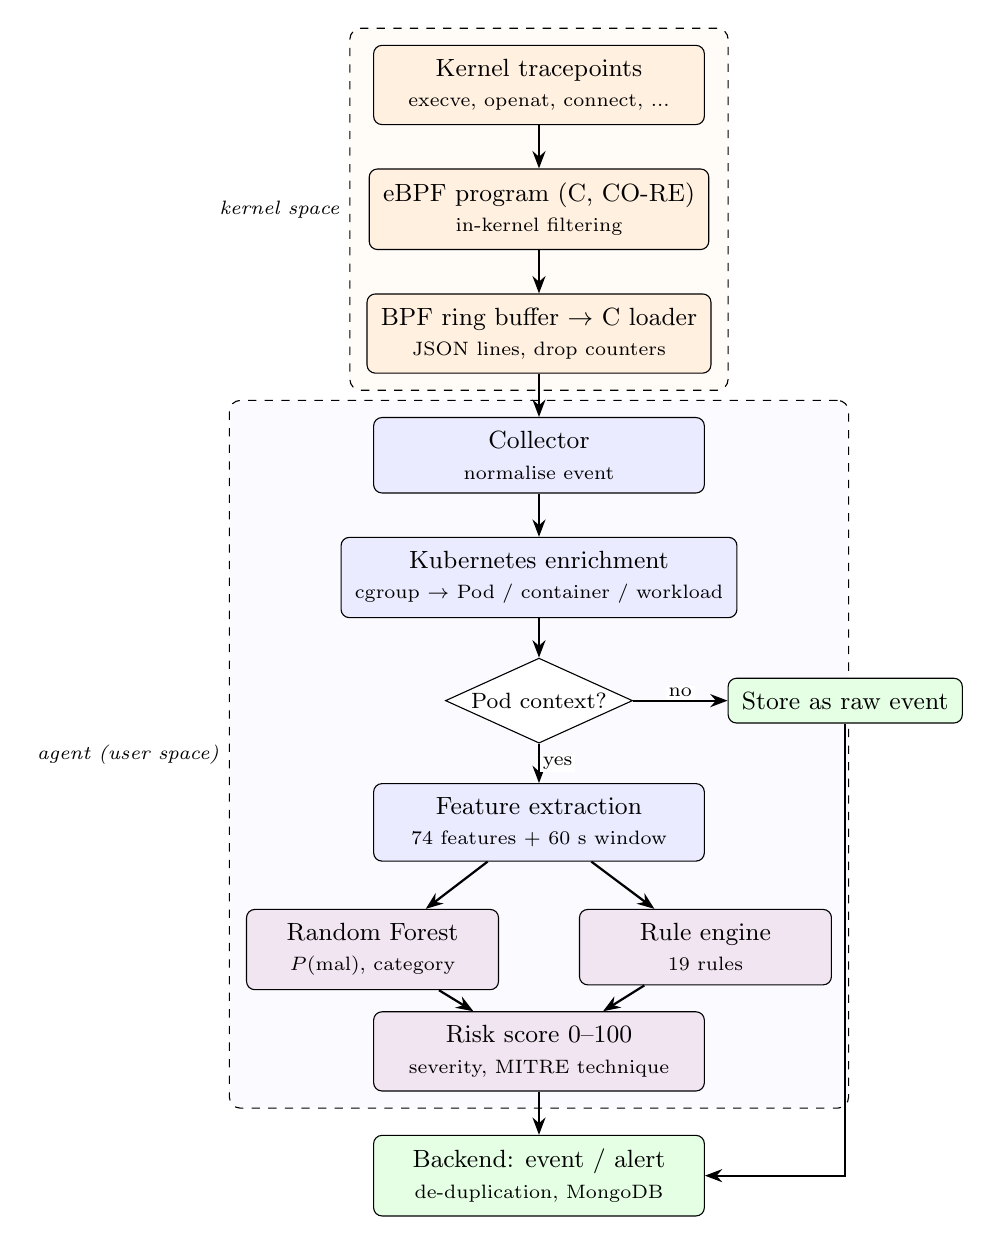
\begin{tikzpicture}[node distance=0.55cm and 0.5cm, every node/.style={font=\small}]
  \node[kbox, minimum width=4.2cm] (k) {Kernel tracepoints\\ \scriptsize execve, openat, connect, ...};
  \node[kbox, below=of k, minimum width=4.2cm] (ebpf) {eBPF program (C, CO-RE)\\ \scriptsize in-kernel filtering};
  \node[kbox, below=of ebpf, minimum width=4.2cm] (rb) {BPF ring buffer $\rightarrow$ C loader\\ \scriptsize JSON lines, drop counters};
  \node[ubox, below=of rb, minimum width=4.2cm] (col) {Collector\\ \scriptsize normalise event};
  \node[ubox, below=of col, minimum width=4.2cm] (enr) {Kubernetes enrichment\\ \scriptsize cgroup $\rightarrow$ Pod / container / workload};
  \node[decision, below=0.5cm of enr] (ctx) {Pod context?};
  \node[dbox, right=1.2cm of ctx] (raw) {Store as raw event};
  \node[ubox, below=0.5cm of ctx, minimum width=4.2cm] (fe) {Feature extraction\\ \scriptsize 74 features + 60 s window};
  \node[mlbox, below left=0.6cm and -1.6cm of fe, minimum width=3.2cm] (rf) {Random Forest\\ \scriptsize $P(\mathrm{mal})$, category};
  \node[mlbox, below right=0.6cm and -1.6cm of fe, minimum width=3.2cm] (rules) {Rule engine\\ \scriptsize 19 rules};
  \node[mlbox, below=1.9cm of fe, minimum width=4.2cm] (risk) {Risk score 0--100\\ \scriptsize severity, MITRE technique};
  \node[dbox, below=of risk, minimum width=4.2cm] (be) {Backend: event / alert\\ \scriptsize de-duplication, MongoDB};

  \draw[arr] (k) -- (ebpf);
  \draw[arr] (ebpf) -- (rb);
  \draw[arr] (rb) -- (col);
  \draw[arr] (col) -- (enr);
  \draw[arr] (enr) -- (ctx);
  \draw[arr] (ctx) -- node[lbl, above]{no} (raw);
  \draw[arr] (ctx) -- node[lbl, right]{yes} (fe);
  \draw[arr] (fe) -- (rf);
  \draw[arr] (fe) -- (rules);
  \draw[arr] (rf) -- (risk);
  \draw[arr] (rules) -- (risk);
  \draw[arr] (risk) -- (be);
  \draw[arr] (raw) |- (be);

  \begin{scope}[on background layer]
    \node[draw, dashed, rounded corners, fill=orange!3, fit=(k)(rb), inner sep=6pt,
          label={[font=\scriptsize\itshape]left:kernel space}] {};
    \node[draw, dashed, rounded corners, fill=blue!2, fit=(col)(risk)(rf)(rules), inner sep=6pt,
          label={[font=\scriptsize\itshape]left:agent (user space)}] {};
  \end{scope}
\end{tikzpicture}
\caption{Processing pipeline of the proposed system}
\label{fig:pipeline}
\end{figure}

\section{Kernel-Level Event Capture with eBPF}

The sensor is an eBPF program (\texttt{bpf/ids.bpf.c}) compiled with clang and loaded
with libbpf using \emph{Compile Once -- Run Everywhere} (CO-RE). CO-RE relocates
kernel structure offsets at load time using the kernel's BTF information, so one binary
runs on any kernel version with BTF, without kernel headers on the node.

The program attaches to the system-call tracepoints in Table~\ref{tab:tracepoints}.
For every event it records the cgroup ID, PID, parent PID, user ID, process and parent
name, and the arguments relevant for that call. Several filters run \emph{inside} the
kernel to reduce overhead: \texttt{openat} events are only emitted for sensitive path
prefixes, \texttt{chmod} only when SUID/SGID or execute bits are set, and
\texttt{execve} is reported on syscall exit so that only \emph{successful} executions are
emitted. Process arguments are copied up to eight arguments of 127 bytes. Events are
written to a BPF ring buffer; if the buffer is full the event is counted in a per-CPU
drop counter, which the agent reports so that data loss is never silent.

\begin{table}[H]
\centering
\caption{Monitored system-call tracepoints}
\label{tab:tracepoints}
\footnotesize
\begin{tabularx}{\textwidth}{l >{\raggedright\arraybackslash}p{5.2cm} >{\raggedright\arraybackslash}X}
\toprule
\textbf{Event type} & \textbf{Tracepoint(s)} & \textbf{Data captured} \\
\midrule
exec    & sys\_enter / sys\_exit\_execve & binary path, argv (8 $\times$ 127 B) \\
open    & sys\_enter\_openat & path, flags (sensitive prefixes only) \\
connect & sys\_enter\_connect & family, port, IPv4/IPv6 address, UNIX path \\
ptrace  & sys\_enter\_ptrace & request, target PID \\
setuid  & sys\_enter\_setuid, sys\_enter\_setresuid & target user ID \\
mount   & sys\_enter\_mount & source, target, filesystem type \\
unshare & sys\_enter\_unshare & namespace flags \\
setns   & sys\_enter\_setns & namespace type \\
chmod   & sys\_enter\_chmod, fchmodat, fchmodat2 & path, mode \\
module  & sys\_enter\_init\_module, finit\_module & module load \\
memfd   & sys\_enter\_memfd\_create & memfd name \\
\midrule
\multicolumn{3}{l}{\textbf{16 tracepoints in total}} \\
\bottomrule
\end{tabularx}
\end{table}

A small C program (\texttt{loader/ids\_loader.c}) loads and attaches the eBPF program,
polls the ring buffer and prints each event as one JSON line on standard output, where
the Python collector reads it.

\section{Kubernetes Enrichment}

Kernel events identify a container only through its \textbf{cgroup ID}. The enrichment
module resolves the cgroup ID to the cgroup path under \texttt{/sys/fs/cgroup}. Regular
expressions extract the \textbf{Pod UID} and the \textbf{container ID} from the path
(for the systemd and cgroupfs layouts used by containerd and Docker). A cache of Pod
objects on the node, refreshed from the Kubernetes API every 15 seconds, maps the Pod
UID to the Pod name, namespace, container name, image, service account and node. The
owning \textbf{workload} (Deployment, StatefulSet, DaemonSet, Job) is derived from owner
references, for example a ReplicaSet \texttt{shop-web-7b955dcf77} belongs to
Deployment \texttt{shop-web}. Events from processes outside any pod (the node itself)
keep an empty namespace and are stored as \emph{raw} events.

\section{Feature Extraction}

The feature module (\texttt{ids\_agent/features.py}) converts an event and its
behaviour window into a vector of \textbf{74 numeric features}. The same module is
imported by the training script and by the live agent, which removes the
train/serve mismatch of the v0 prototype. Table~\ref{tab:features} summarises the
feature groups.

\begin{table}[H]
\centering
\caption{Feature groups (74 features)}
\label{tab:features}
\small
\begin{tabularx}{\textwidth}{>{\raggedright\arraybackslash}p{3.3cm} c >{\raggedright\arraybackslash}X}
\toprule
\textbf{Group} & \textbf{\#} & \textbf{Examples} \\
\midrule
Event type (one-hot) & 11 & ev\_exec, ev\_open, ev\_connect, ev\_mount, ev\_memfd \\
Identity & 2 & uid\_root, ns\_system (platform namespace) \\
Command line & 9 & length, number of arguments, special characters, Shannon entropy, base64 blob, IP literal, URL, \texttt{/dev/tcp} \\
Binary class & 10 & shell, network tool, interpreter, recon tool, container tool, escape tool, package manager, runs from /tmp, hidden, fileless \\
Process lineage & 7 & K8s component, auth binary, debugger, parent is shell / server / interpreter / K8s component \\
Argument patterns & 9 & sensitive path, download, download-and-execute, write to /tmp, SUID, reverse shell, miner, log cleanup, recon \\
File & 2 & sensitivity level of path (0--2), write access \\
Network & 7 & UNIX socket, common / suspicious / high port, private, loopback, link-local destination \\
Privilege & 9 & ptrace attach, setuid to root, user / mount namespace unshare, SUID / exec chmod, benign memfd name, block-device mount, host-path mount \\
Behaviour window & 8 & executions, distinct binaries, connections, distinct destinations, sensitive opens, shells, new binary, shell ratio \\
\bottomrule
\end{tabularx}
\end{table}

\textbf{Command-line entropy.} For a command line $s$ with character frequencies $p_c$,
the Shannon entropy
\begin{equation}
H(s) = -\sum_{c} p_c \log_2 p_c
\end{equation}
is high for encoded or random payloads and low for ordinary commands.

\textbf{Behaviour window.} For each container the agent keeps a sliding window of the
last $W = 60$ seconds of events. The window counts are log-transformed,
$x' = \log(1 + x)$, so that bursts of thousands of events do not dominate. A binary is
marked as \emph{new} if it has not been executed in the same workload before, once a
warm-up period of five minutes has passed; this captures the classic sign of an
intrusion: a container that suddenly runs programs it never ran before.

\section{Random Forest Classifier}

A Random Forest~\cite{breiman2001} is an ensemble of $T$ decision trees, each trained on
a bootstrap sample of the training data with a random subset of features considered at
every split. For an input vector $\mathbf{x}$, every tree $t$ outputs class
probabilities $p_t(c \mid \mathbf{x})$ and the forest averages them:
\begin{equation}
P(c \mid \mathbf{x}) = \frac{1}{T} \sum_{t=1}^{T} p_t(c \mid \mathbf{x}).
\end{equation}
The model is trained on \textbf{ten classes} (benign and nine attack categories). Two
quantities are derived from the output:
\begin{align}
P(\mathrm{mal} \mid \mathbf{x}) &= 1 - P(\mathrm{benign} \mid \mathbf{x}), \\
\hat{c}(\mathbf{x}) &= \arg\max_{c \neq \mathrm{benign}} P(c \mid \mathbf{x}).
\end{align}
An event is an ML detection if $P(\mathrm{mal}) \geq \tau$ with $\tau = 0.5$; in
platform namespaces (for example \texttt{kube-system}) without a matching rule, the
threshold is raised to 0.75 because platform components legitimately perform many
sensitive operations. The predicted attack category $\hat{c}$ selects the MITRE
technique of an ML-only alert.

\textbf{Hyper-parameters:} 150 trees, maximum depth 22, minimum one sample per leaf,
$\sqrt{74}$ features per split, no class weighting, random state 42. Balanced class
weights were tested and rejected: they raised detection to 100\% but increased the
false-positive rate to 4.6\%, because up-weighting nine small attack classes inflates
$P(\mathrm{mal})$.

\section{Rule Engine}

Rules provide high-precision detection of well-known techniques and an explanation
that operators understand. Each rule receives the event and its feature vector and
returns true or false; a failing rule is skipped and never stops the sensor. Platform
components (Kubernetes namespaces such as \texttt{kube-system}, container runtimes,
CoreDNS) are exempted where their normal behaviour would otherwise match.

\begin{longtable}{p{1.0cm} p{6.6cm} p{1.5cm} p{2.2cm}}
\caption{Detection rules}\label{tab:rules}\\
\toprule
\textbf{ID} & \textbf{Rule} & \textbf{Severity} & \textbf{MITRE} \\
\midrule
\endfirsthead
\toprule
\textbf{ID} & \textbf{Rule} & \textbf{Severity} & \textbf{MITRE} \\
\midrule
\endhead
R001 & Reverse-shell command line & High & T1059.004 \\
R002 & Shell / interpreter connecting to a suspicious port & High & T1571 \\
R003 & Service-account token read by a shell tool & High & T1528 \\
R004 & Password database read & High & T1003.008 \\
R005 & Crypto-miner activity (arguments or pool ports) & High & T1496 \\
R006 & Download piped into a shell & High & T1105 \\
R007 & Binary executed from a temp / hidden location & Medium & T1204.002 \\
R008 & Kernel module loaded from a pod & High & T1547.006 \\
R009 & Process injection via ptrace & Medium & T1055.008 \\
R010 & SUID/SGID bit set on a binary & High & T1548.001 \\
R011 & Web / server process spawned a shell or recon tool & Medium & T1190 \\
R012 & Fileless execution (memfd / fd exec) & High & T1620 \\
R013 & Log or shell-history tampering & Medium & T1070 \\
R014 & Container-escape technique (nsenter to PID 1, cgroup / block-device mount, user-namespace unshare, runtime socket, core\_pattern) & High & T1611 \\
R015 & Cloud metadata endpoint access & Medium & T1552.005 \\
R016 & Persistence / authentication file modified & High & T1098 \\
R017 & Kubelet / etcd API accessed from a workload & High & T1210 \\
R018 & Network scanning tool & Medium & T1046 \\
R019 & Privilege escalation to root by a non-auth binary & High & T1068 \\
\bottomrule
\end{longtable}

\section{Risk Scoring and Severity}

ML and rules are combined into a single risk score. Let $H$ be the set of matched
rules, $s(r)$ the score of rule $r$ ($\mathrm{High}=90$, $\mathrm{Medium}=70$,
$\mathrm{Low}=45$) and $m = \mathbb{1}[P(\mathrm{mal}) \geq \tau]$ the ML decision. Then
\begin{equation}
S_0 = \max\Big( m \cdot 100\,P(\mathrm{mal}),\; \max_{r \in H} s(r) \Big)
\end{equation}
and the final score adds context bonuses and penalties and is clipped to $[0, 100]$:
\begin{equation}
S = \mathrm{clip}\big(S_0 + 5\cdot\mathbb{1}[H \neq \emptyset \wedge m]
      + 3\cdot\mathbb{1}[\mathrm{uid}=0] - 10\cdot\mathbb{1}[\mathrm{ns\_system} \wedge H = \emptyset],\; 0,\; 100\big).
\end{equation}
The bonus of 5 rewards agreement of both detectors, running as root adds 3, and an
ML-only verdict in a platform namespace loses 10. The event is \emph{suspicious} if
$H \neq \emptyset$ or $m = 1$. Severity is assigned as
\begin{equation}
\mathrm{severity}(S) =
\begin{cases}
\mathrm{High}   & S \geq 80,\\
\mathrm{Medium} & 60 \leq S < 80,\\
\mathrm{Low}    & S < 60.
\end{cases}
\end{equation}
The alert's category comes from the highest-severity matched rule, or from the ML
prediction $\hat{c}$ if no rule matched. Each alert lists the matched rules, the ML
probability, the MITRE techniques and the full Kubernetes context.

\section{Alert De-duplication}

An attacker who repeats a command, or a loop that runs every second, would otherwise
create hundreds of identical alerts. The agent computes a de-duplication key as a SHA-1
hash of namespace, workload, container, event type, process name, category and the
command line (or path or destination). The backend merges a new alert into an
unresolved alert with the same key seen within the last \textbf{10 minutes}, increments its
\emph{count} and updates its last-seen time and maximum risk score.

\chapter{System Design}

System design describes the structure of the system, the interaction between its
components and the movement of data between them. This chapter presents the overall
architecture, the Kubernetes deployment, UML diagrams (use case, class and sequence),
data flow diagrams and the database design.

\section{System Architecture}

Figure~\ref{fig:architecture} shows the architecture. Each Kubernetes node runs one
privileged \textbf{agent} pod (DaemonSet) that contains the eBPF sensor and the Python
detection pipeline. The agent sends events, alerts, heartbeats and evaluation reports
to the \textbf{FastAPI backend}, which stores them in \textbf{MongoDB}. The \textbf{React
dashboard} reads them through the backend's REST API. All IDS components run in the
dedicated namespace \texttt{ebpf-ids}.

\begin{figure}[H]
\centering
\resizebox{\textwidth}{!}{%
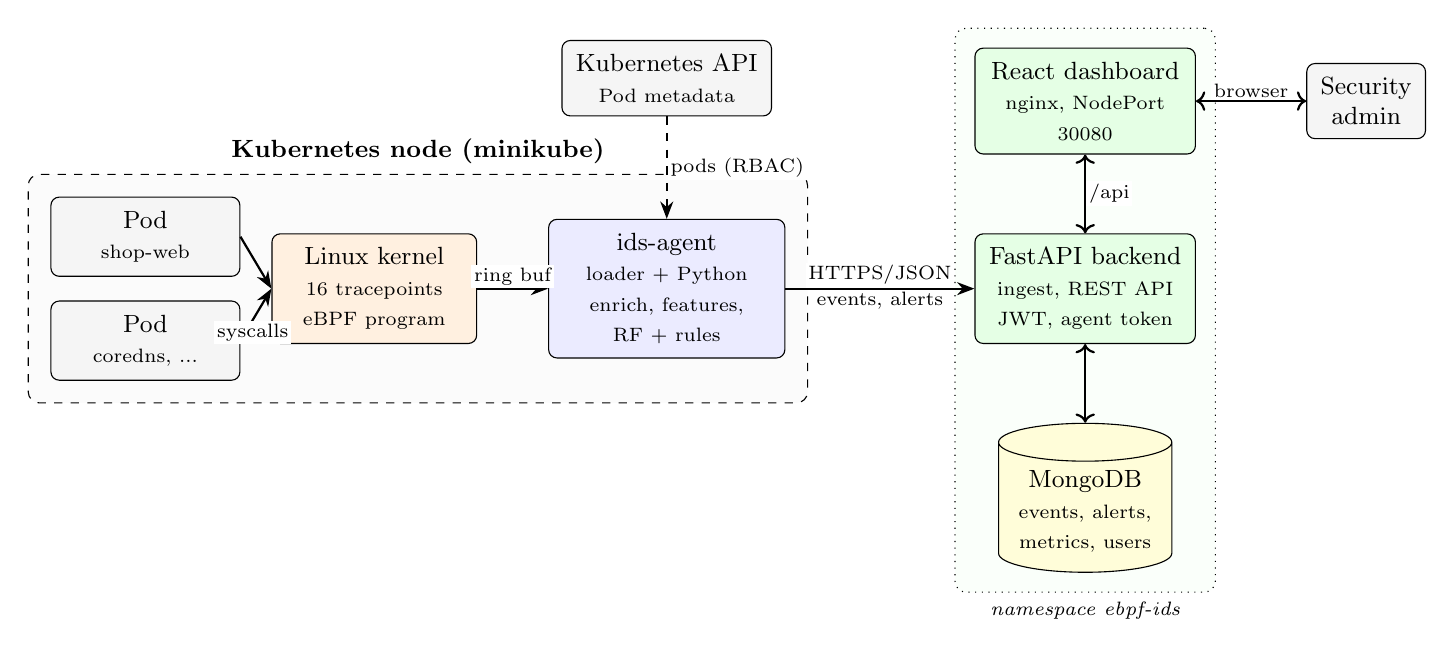
\begin{tikzpicture}[node distance=0.5cm and 0.6cm]
  % node
  \node[box, minimum width=2.4cm, fill=gray!8] (p1) {Pod\\ \scriptsize shop-web};
  \node[box, minimum width=2.4cm, fill=gray!8, below=0.3cm of p1] (p2) {Pod\\ \scriptsize coredns, ...};
  \node[kbox, minimum width=2.6cm, right=1.6cm of $(p1)!0.5!(p2)$] (kern) {Linux kernel\\ \scriptsize 16 tracepoints\\ \scriptsize eBPF program};
  \node[ubox, minimum width=3.0cm, right=0.9cm of kern] (agent) {ids-agent\\ \scriptsize loader + Python\\ \scriptsize enrich, features,\\ \scriptsize RF + rules};
  \begin{scope}[on background layer]
    \node[draw, rounded corners, dashed, fill=gray!3, fit=(p1)(p2)(kern)(agent), inner sep=8pt,
          label={[font=\small\bfseries]above:Kubernetes node (minikube)}] (node) {};
  \end{scope}
  \draw[arr] (p1.east) -- (kern.west);
  \draw[arr] (p2.east) -- node[lbl, below, pos=0.4]{syscalls} (kern.west);
  \draw[arr] (kern) -- node[lbl, above]{ring buf} (agent);

  % control plane
  \node[box, fill=gray!8, above=1.3cm of agent] (api) {Kubernetes API\\ \scriptsize Pod metadata};
  \draw[darr] (api) -- node[lbl, right]{pods (RBAC)} (agent);

  % backend
  \node[dbox, minimum width=2.8cm, right=2.4cm of agent] (be) {FastAPI backend\\ \scriptsize ingest, REST API\\ \scriptsize JWT, agent token};
  \node[db, below=1.0cm of be] (mongo) {MongoDB\\ \scriptsize events, alerts,\\ \scriptsize metrics, users};
  \node[dbox, minimum width=2.8cm, above=1.0cm of be] (fe) {React dashboard\\ \scriptsize nginx, NodePort\\ \scriptsize 30080};
  \node[box, fill=gray!8, right=1.4cm of fe] (user) {Security\\ admin};

  \draw[arr] (agent) -- node[lbl, above]{HTTPS/JSON} node[lbl, below]{events, alerts} (be);
  \draw[arr, <->] (be) -- (mongo);
  \draw[arr, <->] (fe) -- node[lbl, right]{/api} (be);
  \draw[arr, <->] (user) -- node[lbl, above]{browser} (fe);
  \begin{scope}[on background layer]
    \node[draw, rounded corners, dotted, fill=green!2, fit=(be)(mongo)(fe), inner sep=7pt,
          label={[font=\scriptsize\itshape]below:namespace ebpf-ids}] {};
  \end{scope}
\end{tikzpicture}}
\caption{System architecture}
\label{fig:architecture}
\end{figure}

\section{Deployment Design}

The system is deployed with plain Kubernetes manifests (\texttt{infra/k8s/}) and one
script (\texttt{scripts/deploy\_minikube.sh}). Table~\ref{tab:k8sobjects} lists the
Kubernetes objects. The agent needs \texttt{hostPID} and \texttt{privileged} mode to load
eBPF programs and read every process on the node; it is limited by resource requests
(50m CPU, 192 MiB) and limits (1 CPU, 512 MiB), and its service account can only
\emph{get, list} and \emph{watch} pods. Credentials (MongoDB password, JWT secret, agent
token, admin password) are generated randomly at deployment time and stored in the
Kubernetes Secret \texttt{ids-secrets}.

\begin{table}[H]
\centering
\caption{Kubernetes objects of the deployment}
\label{tab:k8sobjects}
\small
\begin{tabularx}{\textwidth}{>{\raggedright\arraybackslash}p{4.4cm} l >{\raggedright\arraybackslash}X}
\toprule
\textbf{Object} & \textbf{Name} & \textbf{Purpose} \\
\midrule
Namespace & ebpf-ids & Isolates all IDS components \\
DaemonSet & ids-agent & One eBPF sensor + detector per node \\
ServiceAccount, ClusterRole, Binding & ids-agent & Read-only access to pods \\
Deployment + Service & ids-backend & FastAPI REST API (port 8000) \\
Deployment + Service & ids-frontend & React dashboard (NodePort 30080) \\
Deployment + Service + PVC & ids-mongodb & MongoDB 7.0 with persistent volume \\
Secret & ids-secrets & Random credentials and tokens \\
Deployment (test) & ids-demo/shop-web & Victim workload for evaluation \\
\bottomrule
\end{tabularx}
\end{table}

\section{UML Diagrams}

\subsection{Use Case Diagram}

Figure~\ref{fig:usecase} shows the actors and use cases. The \emph{security
administrator} uses the dashboard and the evaluation script. The \emph{eBPF agent} is a
system actor that monitors workloads and reports to the backend. A \emph{workload
process} (possibly controlled by an attacker) triggers kernel events without knowing it
is observed.

\begin{figure}[H]
\centering
\resizebox{0.95\textwidth}{!}{%
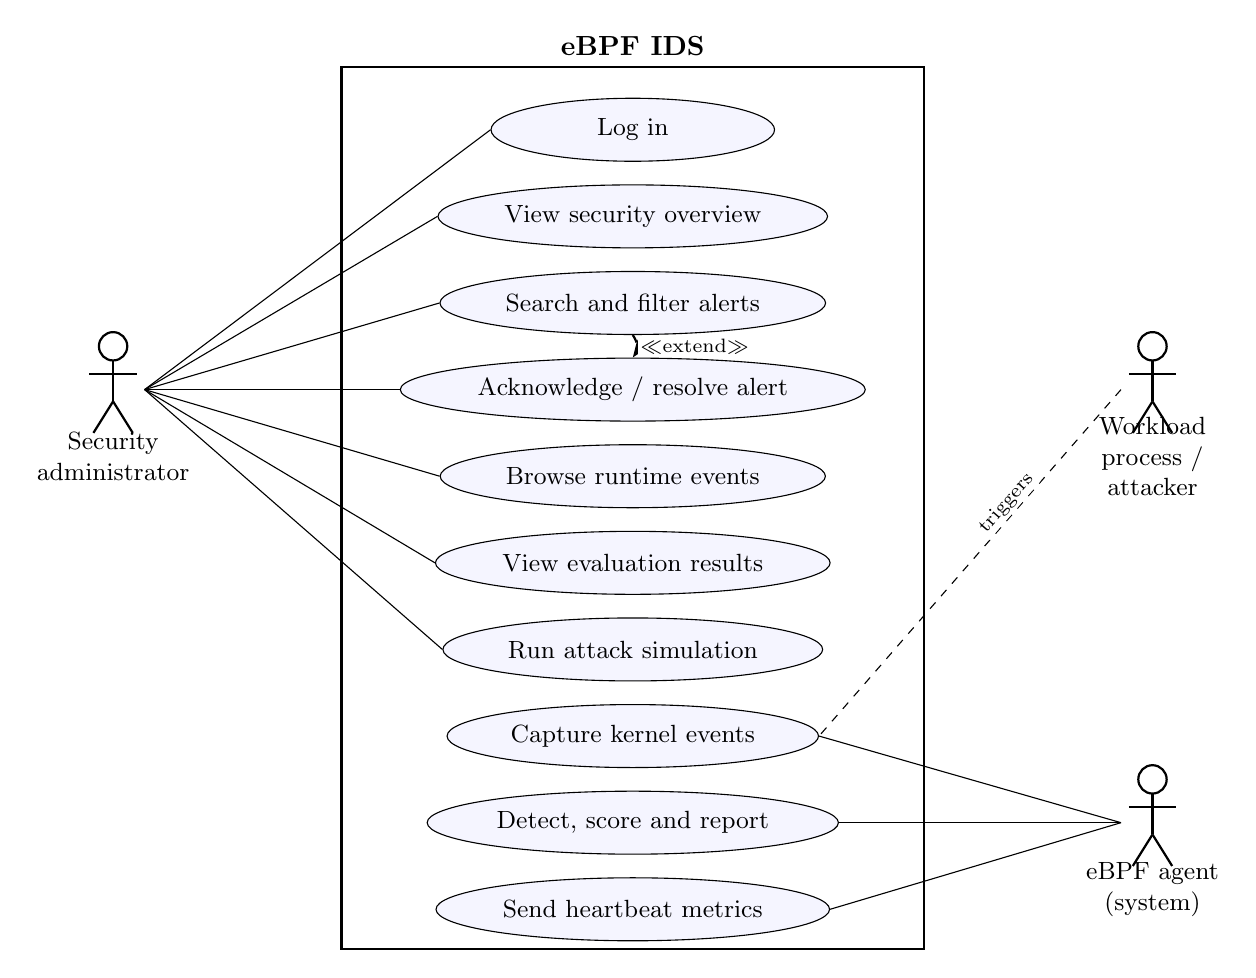
\begin{tikzpicture}[uc/.style={draw, ellipse, align=center, font=\small, minimum width=3.6cm, minimum height=0.8cm, fill=blue!4},
                    actor/.style={align=center, font=\small}]
  \newcommand{\stick}[2]{%
    \begin{scope}[shift={#1}]
      \draw[thick] (0,0.55) circle (0.18);
      \draw[thick] (0,0.37) -- (0,-0.15);
      \draw[thick] (-0.3,0.2) -- (0.3,0.2);
      \draw[thick] (0,-0.15) -- (-0.25,-0.55);
      \draw[thick] (0,-0.15) -- (0.25,-0.55);
      \node[actor] at (0,-0.85) {#2};
    \end{scope}}
  \node[draw, thick, minimum width=7.4cm, minimum height=11.2cm, label={[font=\bfseries]above:eBPF IDS}] (sys) at (0,0) {};
  \node[uc] (u1) at (0,4.8) {Log in};
  \node[uc] (u2) at (0,3.7) {View security overview};
  \node[uc] (u3) at (0,2.6) {Search and filter alerts};
  \node[uc] (u4) at (0,1.5) {Acknowledge / resolve alert};
  \node[uc] (u5) at (0,0.4) {Browse runtime events};
  \node[uc] (u6) at (0,-0.7) {View evaluation results};
  \node[uc] (u7) at (0,-1.8) {Run attack simulation};
  \node[uc] (u8) at (0,-2.9) {Capture kernel events};
  \node[uc] (u9) at (0,-4.0) {Detect, score and report};
  \node[uc] (u10) at (0,-5.1) {Send heartbeat metrics};

  \stick{(-6.6,1.5)}{Security\\administrator}
  \stick{(6.6,-4.0)}{eBPF agent\\(system)}
  \stick{(6.6,1.5)}{Workload\\process /\\attacker}

  \foreach \u in {u1,u2,u3,u4,u5,u6,u7} \draw (-6.2,1.5) -- (\u.west);
  \foreach \u in {u8,u9,u10} \draw (6.2,-4.0) -- (\u.east);
  \draw[dashed] (6.2,1.5) -- node[lbl, sloped, above, pos=0.35]{triggers} (u8.east);
  \draw[darr] (u3.south) to[bend left=35] node[lbl, right]{\scriptsize $\ll$extend$\gg$} (u4.north);
\end{tikzpicture}}
\caption{Use case diagram}
\label{fig:usecase}
\end{figure}

\subsection{Class Diagram}

Figure~\ref{fig:class} shows the main classes of the agent and the documents stored by
the backend. The \texttt{Agent} orchestrates a \texttt{Collector} (reads the loader's
JSON stream), a \texttt{K8sEnricher} (with \texttt{CgroupResolver} and
\texttt{KubeClient}), a \texttt{BehaviorTracker}, the \texttt{Detector} (Random Forest
and rules), a \texttt{Shipper} (batched HTTP delivery) and \texttt{Metrics} (CPU, memory,
latency, drops).

\begin{figure}[H]
\centering
\resizebox{\textwidth}{!}{%
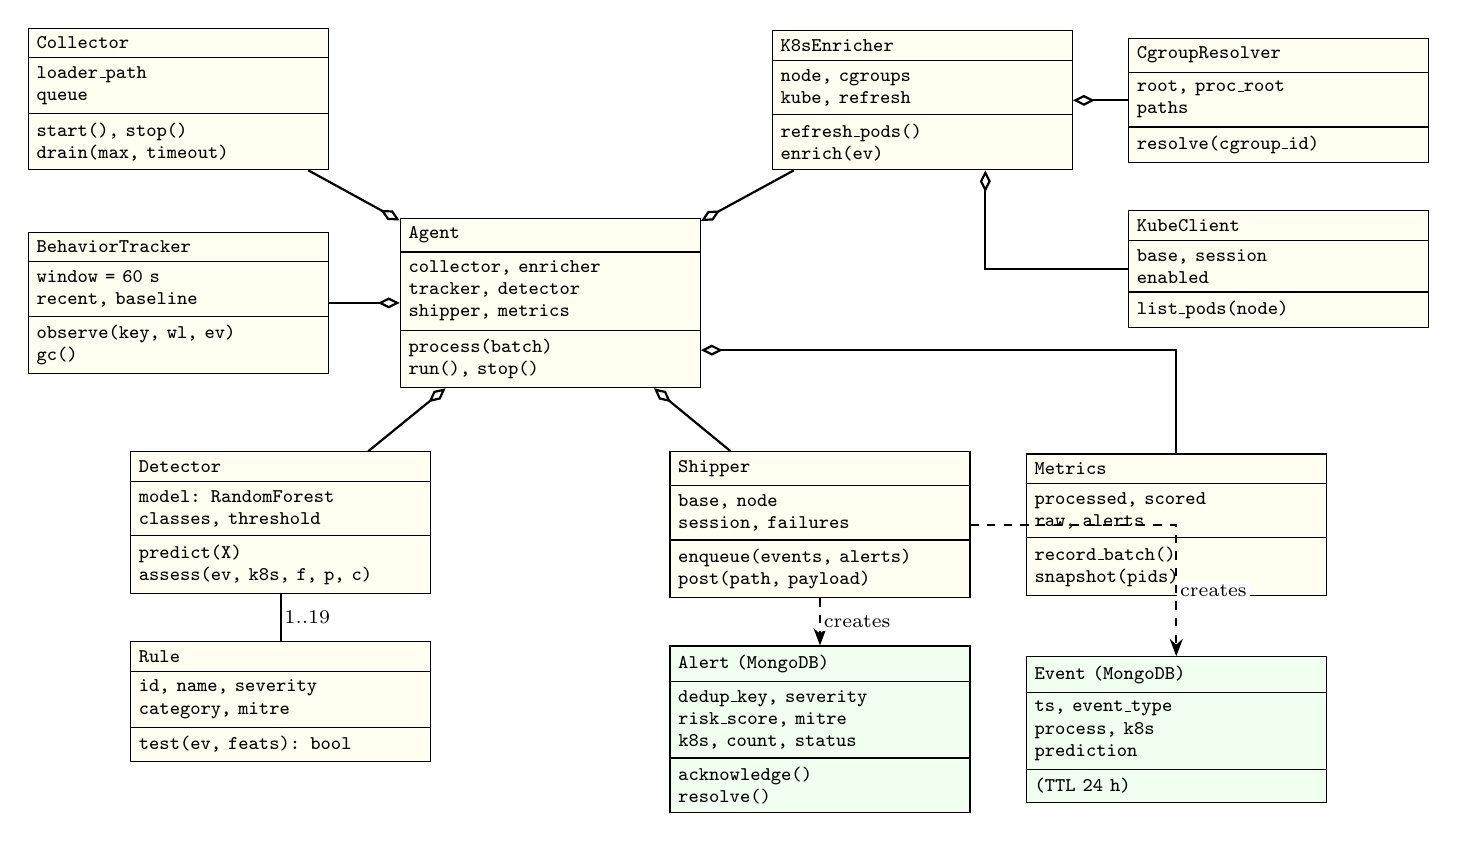
\begin{tikzpicture}[cls/.style={draw, rectangle split, rectangle split parts=3, align=left,
                    font=\scriptsize\ttfamily, fill=yellow!6, inner sep=3pt, text width=3.6cm},
                    node distance=0.7cm and 0.7cm]
  \node[cls] (agent) {\textbf{Agent}
    \nodepart{second} collector, enricher\\ tracker, detector\\ shipper, metrics
    \nodepart{third} process(batch)\\ run(), stop()};
  \node[cls, above left=0.6cm and 0.9cm of agent] (col) {\textbf{Collector}
    \nodepart{second} loader\_path\\ queue
    \nodepart{third} start(), stop()\\ drain(max, timeout)};
  \node[cls, above right=0.6cm and 0.9cm of agent] (enr) {\textbf{K8sEnricher}
    \nodepart{second} node, cgroups\\ kube, refresh
    \nodepart{third} refresh\_pods()\\ enrich(ev)};
  \node[cls, right=0.7cm of enr] (cg) {\textbf{CgroupResolver}
    \nodepart{second} root, proc\_root\\ paths
    \nodepart{third} resolve(cgroup\_id)};
  \node[cls, below=0.6cm of cg] (kc) {\textbf{KubeClient}
    \nodepart{second} base, session\\ enabled
    \nodepart{third} list\_pods(node)};
  \node[cls, left=0.9cm of agent] (bt) {\textbf{BehaviorTracker}
    \nodepart{second} window = 60 s\\ recent, baseline
    \nodepart{third} observe(key, wl, ev)\\ gc()};
  \node[cls, below left=0.8cm and -0.4cm of agent] (det) {\textbf{Detector}
    \nodepart{second} model: RandomForest\\ classes, threshold
    \nodepart{third} predict(X)\\ assess(ev, k8s, f, p, c)};
  \node[cls, below right=0.8cm and -0.4cm of agent] (sh) {\textbf{Shipper}
    \nodepart{second} base, node\\ session, failures
    \nodepart{third} enqueue(events, alerts)\\ post(path, payload)};
  \node[cls, below=0.6cm of det] (rule) {\textbf{Rule}
    \nodepart{second} id, name, severity\\ category, mitre
    \nodepart{third} test(ev, feats): bool};
  \node[cls, right=0.7cm of sh] (met) {\textbf{Metrics}
    \nodepart{second} processed, scored\\ raw, alerts
    \nodepart{third} record\_batch()\\ snapshot(pids)};
  \node[cls, below=0.6cm of sh, fill=green!6] (alert) {\textbf{Alert} (MongoDB)
    \nodepart{second} dedup\_key, severity\\ risk\_score, mitre\\ k8s, count, status
    \nodepart{third} acknowledge()\\ resolve()};
  \node[cls, right=0.7cm of alert, fill=green!6] (event) {\textbf{Event} (MongoDB)
    \nodepart{second} ts, event\_type\\ process, k8s\\ prediction
    \nodepart{third} (TTL 24 h)};

  \draw[-{Diamond[open]}, thick] (col) -- (agent);
  \draw[-{Diamond[open]}, thick] (enr) -- (agent);
  \draw[-{Diamond[open]}, thick] (bt) -- (agent);
  \draw[-{Diamond[open]}, thick] (det) -- (agent);
  \draw[-{Diamond[open]}, thick] (sh) -- (agent);
  \draw[-{Diamond[open]}, thick] (met.north) |- ($(agent.east)+(0,-0.6)$);
  \draw[-{Diamond[open]}, thick] (cg) -- (enr);
  \draw[-{Diamond[open]}, thick] (kc.west) -| ($(enr.south)+(0.8,0)$);
  \draw[thick] (det) -- node[lbl, right]{1..19} (rule);
  \draw[darr] (sh) -- node[lbl, right]{creates} (alert);
  \draw[darr] (sh.east) -| node[lbl, near end, right]{creates} (event.north);
\end{tikzpicture}}
\caption{Class diagram of the agent and stored documents}
\label{fig:class}
\end{figure}

\subsection{Sequence Diagram}

Figure~\ref{fig:sequence} shows the sequence of interactions when an attacker opens a
reverse shell inside a pod and the administrator investigates the alert.

\begin{figure}[H]
\centering
\resizebox{\textwidth}{!}{%
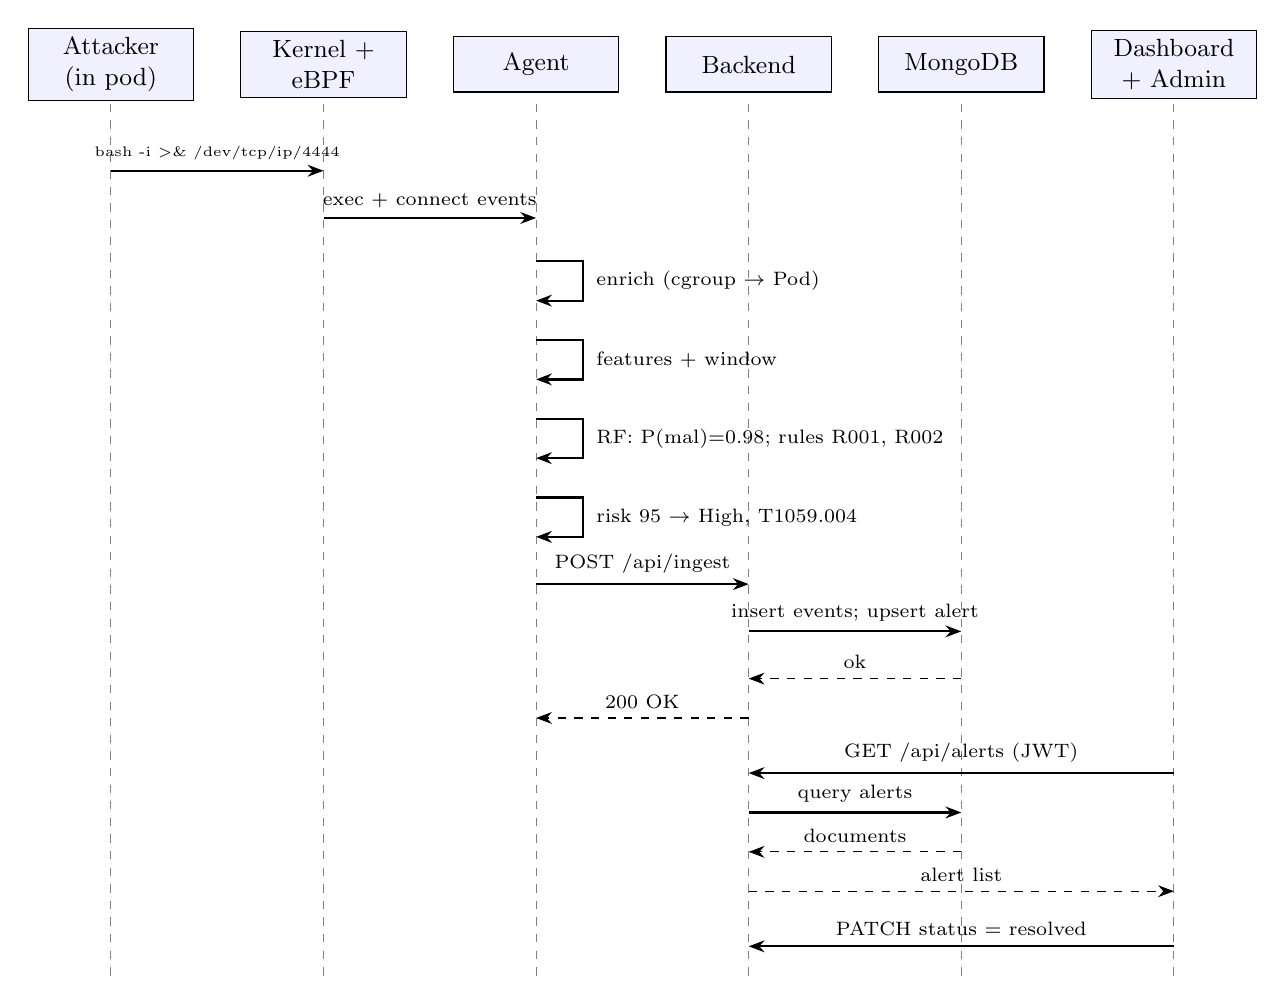
\begin{tikzpicture}[ll/.style={draw, fill=blue!6, font=\small, minimum width=2.1cm, minimum height=0.7cm, align=center},
                    msg/.style={-{Stealth[length=2mm]}, thick},
                    ret/.style={-{Stealth[length=2mm]}, dashed},
                    m/.style={font=\scriptsize, above}]
  \def\H{-11.6}
  \foreach \x/\n/\t in {0/a/Attacker\\(in pod), 2.7/k/Kernel +\\eBPF, 5.4/g/Agent, 8.1/b/Backend, 10.8/d/MongoDB, 13.5/u/Dashboard\\+ Admin} {
    \node[ll] (\n) at (\x,0) {\t};
    \draw[dashed, gray] (\x,-0.5) -- (\x,\H);
  }
  \draw[msg] (0,-1.35) -- node[m, font=\tiny]{bash -i \textgreater\& /dev/tcp/ip/4444} (2.7,-1.35);
  \draw[msg] (2.7,-1.95) -- node[m]{exec + connect events} (5.4,-1.95);
  \draw[msg] (5.4,-2.5) -- ++(0.6,0) -- node[m, right, xshift=1pt]{enrich (cgroup $\rightarrow$ Pod)} ++(0,-0.5) -- ++(-0.6,0);
  \draw[msg] (5.4,-3.5) -- ++(0.6,0) -- node[m, right, xshift=1pt]{features + window} ++(0,-0.5) -- ++(-0.6,0);
  \draw[msg] (5.4,-4.5) -- ++(0.6,0) -- node[m, right, xshift=1pt]{RF: P(mal)=0.98; rules R001, R002} ++(0,-0.5) -- ++(-0.6,0);
  \draw[msg] (5.4,-5.5) -- ++(0.6,0) -- node[m, right, xshift=1pt]{risk 95 $\rightarrow$ High, T1059.004} ++(0,-0.5) -- ++(-0.6,0);
  \draw[msg] (5.4,-6.6) -- node[m]{POST /api/ingest} (8.1,-6.6);
  \draw[msg] (8.1,-7.2) -- node[m]{insert events; upsert alert} (10.8,-7.2);
  \draw[ret] (10.8,-7.8) -- node[m]{ok} (8.1,-7.8);
  \draw[ret] (8.1,-8.3) -- node[m]{200 OK} (5.4,-8.3);
  \draw[msg] (13.5,-9.0) -- node[m]{GET /api/alerts (JWT)} (8.1,-9.0);
  \draw[msg] (8.1,-9.5) -- node[m]{query alerts} (10.8,-9.5);
  \draw[ret] (10.8,-10.0) -- node[m]{documents} (8.1,-10.0);
  \draw[ret] (8.1,-10.5) -- node[m]{alert list} (13.5,-10.5);
  \draw[msg] (13.5,-11.2) -- node[m]{PATCH status = resolved} (8.1,-11.2);
\end{tikzpicture}}
\caption{Sequence diagram: detection of a reverse shell}
\label{fig:sequence}
\end{figure}

\section{Data Flow Diagrams}

\subsection{Level 0 (Context Diagram)}

\begin{figure}[H]
\centering
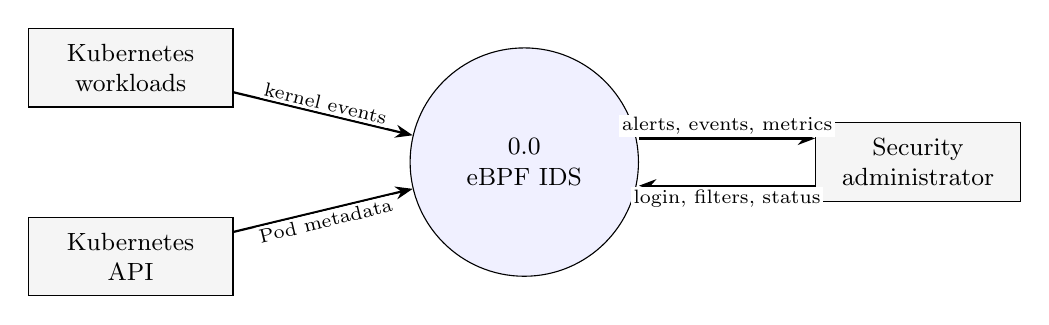
\begin{tikzpicture}[ext/.style={draw, rectangle, font=\small, align=center, minimum width=2.6cm, minimum height=1cm, fill=gray!8},
                    proc/.style={draw, circle, font=\small, align=center, minimum size=2.9cm, fill=blue!6}]
  \node[proc] (p) at (0,0) {0.0\\ eBPF IDS};
  \node[ext] (w) at (-5,1.2) {Kubernetes\\ workloads};
  \node[ext] (k) at (-5,-1.2) {Kubernetes\\ API};
  \node[ext] (a) at (5,0) {Security\\ administrator};
  \draw[arr] (w) -- node[lbl, sloped, above]{kernel events} (p);
  \draw[arr] (k) -- node[lbl, sloped, below]{Pod metadata} (p);
  \draw[arr] ([yshift=0.3cm]p.east) -- node[lbl, above]{alerts, events, metrics} ([yshift=0.3cm]a.west);
  \draw[arr] ([yshift=-0.3cm]a.west) -- node[lbl, below]{login, filters, status} ([yshift=-0.3cm]p.east);
\end{tikzpicture}
\caption{Data flow diagram -- level 0}
\label{fig:dfd0}
\end{figure}

\subsection{Level 1}

\begin{figure}[H]
\centering
\resizebox{\textwidth}{!}{%
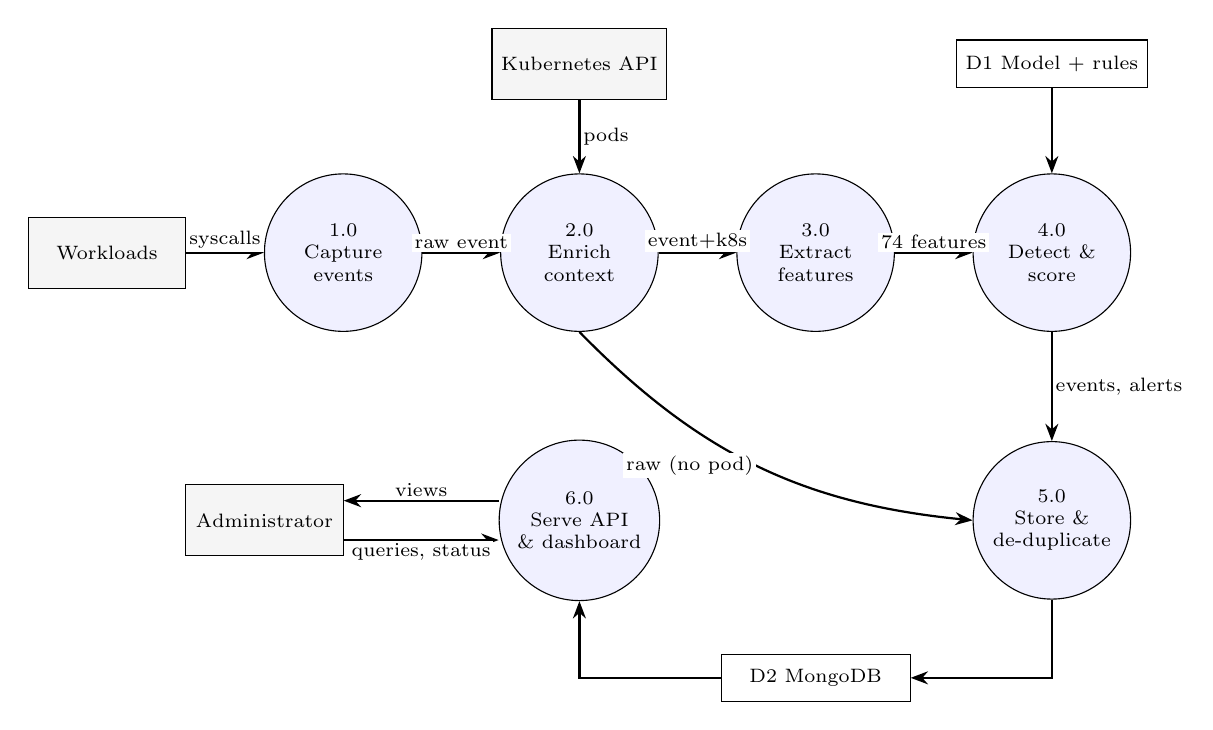
\begin{tikzpicture}[proc/.style={draw, circle, font=\scriptsize, align=center, minimum size=2.0cm, fill=blue!6},
                    store/.style={draw, font=\scriptsize, minimum width=2.4cm, minimum height=0.6cm, path picture={\draw (path picture bounding box.north west) -- (path picture bounding box.south west);}},
                    ext/.style={draw, rectangle, font=\scriptsize, align=center, minimum width=2.0cm, minimum height=0.9cm, fill=gray!8}]
  \node[ext] (w) at (0,0) {Workloads};
  \node[proc] (p1) at (3,0) {1.0\\ Capture\\ events};
  \node[proc] (p2) at (6,0) {2.0\\ Enrich\\ context};
  \node[proc] (p3) at (9,0) {3.0\\ Extract\\ features};
  \node[proc] (p4) at (12,0) {4.0\\ Detect \&\\ score};
  \node[proc] (p5) at (12,-3.4) {5.0\\ Store \&\\ de-duplicate};
  \node[proc] (p6) at (6,-3.4) {6.0\\ Serve API\\ \& dashboard};
  \node[ext] (k8s) at (6,2.4) {Kubernetes API};
  \node[store] (model) at (12,2.4) {D1 Model + rules};
  \node[store] (db) at (9,-5.4) {D2 MongoDB};
  \node[ext] (adm) at (2,-3.4) {Administrator};

  \draw[arr] (w) -- node[lbl, above]{syscalls} (p1);
  \draw[arr] (p1) -- node[lbl, above]{raw event} (p2);
  \draw[arr] (k8s) -- node[lbl, right]{pods} (p2);
  \draw[arr] (p2) -- node[lbl, above]{event+k8s} (p3);
  \draw[arr] (p3) -- node[lbl, above]{74 features} (p4);
  \draw[arr] (model) -- (p4);
  \draw[arr] (p4) -- node[lbl, right]{events, alerts} (p5);
  \draw[arr] (p5) |- (db);
  \draw[arr] (db) -| (p6);
  \draw[arr] ([yshift=0.25cm]p6.west) -- node[lbl, above]{views} ([yshift=0.25cm]adm.east);
  \draw[arr] ([yshift=-0.25cm]adm.east) -- node[lbl, below]{queries, status} ([yshift=-0.25cm]p6.west);
  \draw[arr] (p2.south) to[bend right=20] node[lbl, left]{raw (no pod)} (p5.west);
\end{tikzpicture}}
\caption{Data flow diagram -- level 1}
\label{fig:dfd1}
\end{figure}

\section{Database Design}

MongoDB stores five collections in the database \texttt{ebpf\_ids}
(Table~\ref{tab:collections}). Time-to-live (TTL) indexes delete old documents
automatically, and compound indexes support the dashboard's filters by namespace,
verdict, event type and severity.

\begin{table}[H]
\centering
\caption{MongoDB collections}
\label{tab:collections}
\small
\begin{tabularx}{\textwidth}{l >{\raggedright\arraybackslash}X >{\raggedright\arraybackslash}p{3.6cm}}
\toprule
\textbf{Collection} & \textbf{Main fields} & \textbf{Indexes} \\
\midrule
events & ts, event\_type, process (comm, parent, path, cmdline, uid), network (daddr, dport), k8s (namespace, pod, container, workload, node), prediction (label, probability, category) & TTL 24 h; namespace+ts; label+ts; type+ts \\
alerts & dedup\_key, title, category, severity, risk\_score, probability, rules, mitre, tactic, k8s, last\_event, count, status, first\_seen, last\_seen & TTL 30 days; dedup\_key+status; severity; namespace \\
metrics & node, cpu\_percent, rss\_mb, events\_per\_sec, latency avg / p95, kernel drops, ts & TTL 24 h; node+ts \\
evaluations & kind (offline / live), model\_version, report & -- \\
users & username, role, password\_hash (bcrypt) & unique username \\
\bottomrule
\end{tabularx}
\end{table}

\chapter{Implementation}

This chapter describes how the design was implemented: the project structure, the
technologies used, each module, the deployment procedure and the user interface.

\section{Project Structure}

The project is organised as a monorepo with one directory per service, the ML
pipeline, Kubernetes manifests and the evaluation tooling.

\begin{lstlisting}[basicstyle=\ttfamily\scriptsize]
SecureSME-Platform/
+-- services/
|   +-- ebpf-agent/
|   |   +-- bpf/ids.bpf.c, ids.h     # eBPF kernel program (C, CO-RE)
|   |   +-- loader/ids_loader.c      # libbpf loader, ring buffer -> JSON lines
|   |   +-- ids_agent/               # Python pipeline
|   |   |   +-- collector.py         #   read + normalise kernel events
|   |   |   +-- enrichment.py        #   cgroup -> Pod / container / workload
|   |   |   +-- features.py          #   74 features + behaviour window
|   |   |   +-- detector.py          #   Random Forest + risk scoring
|   |   |   +-- rules.py             #   19 detection rules
|   |   |   +-- shipper.py, metrics.py, __main__.py
|   |   +-- tests/                   # agent unit tests
|   |   +-- Dockerfile               # multi-stage: compile eBPF, Python runtime
|   +-- backend/                     # FastAPI + MongoDB REST API (app/, tests/)
|   +-- frontend/                    # React + Tailwind + Recharts dashboard
+-- ml/
|   +-- generate_dataset.py          # synthetic runtime-telemetry dataset
|   +-- convert_external.py          # BETH / Tetragon -> project schema
|   +-- build_final_dataset.py       # final train.csv / test.csv
|   +-- train_model.py               # training + offline evaluation
|   +-- evaluate_model.py            # test-set evaluation
|   +-- model/                       # ids_model.joblib, evaluation.json
+-- infra/k8s/                       # namespace, MongoDB, backend, frontend, agent
+-- evaluation/                      # victim workload + run_live_eval.py + results
+-- scripts/deploy_minikube.sh       # build images and deploy to minikube
+-- README.md, JOURNAL.md
\end{lstlisting}

\section{Technologies Used}

\begin{table}[H]
\centering
\caption{Technologies used}
\label{tab:tech}
\small
\begin{tabularx}{\textwidth}{>{\raggedright\arraybackslash}p{3.2cm} >{\raggedright\arraybackslash}p{4.0cm} >{\raggedright\arraybackslash}X}
\toprule
\textbf{Layer} & \textbf{Technology} & \textbf{Use} \\
\midrule
Kernel sensor & eBPF, C, clang, libbpf CO-RE, BTF & Tracepoint programs, in-kernel filtering, ring buffer \\
Agent & Python 3.12, NumPy, scikit-learn 1.6, joblib, requests & Enrichment, features, inference, shipping \\
Machine learning & scikit-learn Random Forest, pandas & Training and evaluation \\
Backend & FastAPI, Uvicorn, PyMongo (async), PyJWT, bcrypt & REST API, authentication \\
Database & MongoDB 7.0 & Events, alerts, metrics, users \\
Frontend & React 18, Vite, Tailwind CSS, Recharts, React Router, Axios, lucide-react & Dashboard \\
Platform & Docker, Kubernetes, minikube, kubectl & Packaging and deployment \\
Testing & pytest, Playwright & Unit, API and UI tests \\
Tools & VS Code, Git, GitHub, Ubuntu Linux & Development \\
\bottomrule
\end{tabularx}
\end{table}

\section{Module Description}

\subsection{eBPF Program and Loader}

\textbf{Purpose:} capture security-relevant kernel events with minimal overhead.

\textbf{Implementation highlights:}
\begin{itemize}
    \item One tracepoint handler per system call fills a common event structure
          (\texttt{ids.h}) with cgroup ID, PIDs, UID, process names and arguments.
    \item \texttt{execve} arguments are read on entry and the event is emitted on exit
          only if the call succeeded, so failed executions do not create noise.
    \item File-open events are filtered in the kernel by a list of sensitive path
          prefixes (for example \texttt{/etc/shadow}, \texttt{/var/run/secrets},
          \texttt{/root/.ssh}, runtime sockets).
    \item Events go to a BPF ring buffer; a per-CPU array counts emitted and dropped
          events.
    \item The loader (\texttt{ids\_loader.c}) opens, loads and attaches the CO-RE object
          with libbpf and writes one JSON line per event to standard output. The image is
          built in a multi-stage Dockerfile, so clang and libbpf are not needed on the
          node.
\end{itemize}

\subsection{Python Agent}

\textbf{Purpose:} turn raw kernel events into scored, enriched events and alerts.

\textbf{Implementation highlights:}
\begin{itemize}
    \item \textbf{Collector} starts the loader as a sub-process, reads its JSON lines on a
          thread and normalises them into event dictionaries.
    \item \textbf{K8sEnricher} resolves the cgroup ID to Pod and container and refreshes
          the list of pods on the node from the Kubernetes API.
    \item \textbf{BehaviorTracker} maintains the 60-second window per container and the
          set of known binaries per workload.
    \item \textbf{Detector} loads the model bundle, verifies that the model's feature
          names match the agent's feature module, scores events in batches and combines
          the result with the rules into a decision (Section~5.6).
    \item \textbf{Shipper} sends events and alerts in batches with retries, using the
          shared agent token; \textbf{Metrics} reports CPU, memory, throughput, latency
          and kernel drops every 10 seconds as a heartbeat.
\end{itemize}

Listing~\ref{lst:rules} shows how rules are expressed. Each rule is a small predicate
over the event and its features, with an explicit severity, category and MITRE
technique.

\begin{lstlisting}[language=Python, caption={Excerpt of the rule definitions (\texttt{rules.py})}, label={lst:rules}]
Rule("R001", "Reverse shell command line", "High", "reverse_shell", "T1059.004",
     lambda e, f: f["args_reverse_shell"] and e["event_type"] == "exec"),
Rule("R003", "Service-account token read by a shell tool", "High",
     "credential_access", "T1528",
     lambda e, f: f["ev_open"] and e["path"].startswith(("/var/run/secrets", "/run/secrets"))
     and e["comm"] in TOOLS_FOR_TOKEN_THEFT and not f["ns_system"]),
Rule("R017", "Kubelet / etcd API accessed from a workload", "High",
     "lateral_movement", "T1210",
     lambda e, f: f["ev_connect"] and e.get("dport") in CONTROL_PLANE_PORTS
     and not _platform(f)),
\end{lstlisting}

\subsection{Machine-Learning Pipeline}

\begin{itemize}
    \item \texttt{generate\_dataset.py} creates the labelled synthetic dataset
          (Chapter~4).
    \item \texttt{convert\_external.py} converts BETH and Tetragon data, using all CPU cores
          and an incremental version of the behaviour window that gives identical results
          to the agent's window but in constant time per event.
    \item \texttt{build\_final\_dataset.py} builds \texttt{train.csv} and \texttt{test.csv}
          with the host-based split.
    \item \texttt{train\_model.py} extracts features with the agent's own module, trains the
          Random Forest and writes the model bundle and \texttt{evaluation.json}
          (hold-out, edge cases, unseen template families, 5-fold cross-validation,
          Isolation Forest baseline, latency, feature importance).
    \item \texttt{evaluate\_model.py} reports binary and multi-class metrics, per-source
          results, a threshold sweep and the train/test overlap on any test file.
\end{itemize}

\subsection{Backend (FastAPI)}

The backend exposes the REST API in Table~\ref{tab:api}. Dashboard endpoints require a
JWT obtained from the login endpoint; agent endpoints require the shared agent token.
On start-up the backend creates the MongoDB indexes and the admin user (with a bcrypt
password hash) from the Kubernetes Secret.

\begin{table}[H]
\centering
\caption{REST API endpoints}
\label{tab:api}
\small
\begin{tabularx}{\textwidth}{l >{\ttfamily}l l >{\raggedright\arraybackslash}X}
\toprule
\textbf{Method} & \normalfont\textbf{Path} & \textbf{Auth} & \textbf{Purpose} \\
\midrule
POST  & /api/auth/login & -- & Obtain a JWT \\
GET   & /api/auth/me & JWT & Current user \\
POST  & /api/ingest & Agent token & Batch of events and alerts \\
POST  & /api/agent/heartbeat & Agent token & CPU, memory, latency, drops \\
POST  & /api/agent/evaluation & Agent token & Offline model report \\
GET   & /api/events & JWT & Search / filter events \\
GET   & /api/alerts & JWT & Search / filter alerts \\
GET   & /api/alerts/\{id\} & JWT & Alert details \\
PATCH & /api/alerts/\{id\} & JWT & Acknowledge / resolve \\
GET   & /api/stats & JWT & Overview statistics \\
GET   & /api/namespaces & JWT & Namespaces for filters \\
GET   & /api/agents & JWT & Agent status \\
GET   & /api/evaluation & JWT & Offline and live evaluation \\
POST  & /api/evaluation/live & JWT & Store live evaluation result \\
GET   & /healthz & -- & Liveness / readiness probe \\
\bottomrule
\end{tabularx}
\end{table}

\subsection{Frontend (React Dashboard)}

The dashboard is a single-page React application built with Vite, styled with Tailwind
CSS and charted with Recharts. It is served by nginx, which also proxies
\texttt{/api} to the backend. Its pages are:
\begin{itemize}
    \item \textbf{Login} -- username and password, JWT stored in the browser.
    \item \textbf{Overview} -- kernel events, open alerts, high-severity count, pods
          monitored, agent overhead, detection latency, timeline, severity distribution,
          attack categories, event types, riskiest pods and MITRE techniques.
    \item \textbf{Alerts} -- search and filters (severity, status, namespace, category);
          a detail panel with risk assessment, rules, MITRE technique, Kubernetes context
          and the kernel event; acknowledge and resolve actions.
    \item \textbf{Events} -- live stream of all kernel events with verdict, filters and
          pause.
    \item \textbf{Evaluation} -- live agent overhead and latency, attack-simulation
          results, model benchmarks, confusion matrix, per-category detection and feature
          importance.
\end{itemize}

\section{Deployment}

The complete system is deployed to minikube with the following commands:
\begin{lstlisting}[language=bash]
python3 -m venv .venv && .venv/bin/pip install -r requirements-dev.txt
.venv/bin/python ml/generate_dataset.py && .venv/bin/python ml/train_model.py
minikube start --driver=docker --cpus=2 --memory=3072
./scripts/deploy_minikube.sh        # build images, create Secret, deploy, wait
\end{lstlisting}

The deployment script builds the three images, loads them into minikube, creates the
namespace and a Secret with random credentials, applies the manifests and waits for
the rollouts. Listing~\ref{lst:pods} shows the running system.

\begin{lstlisting}[caption={Running pods and agent start-up log}, label={lst:pods}, basicstyle=\ttfamily\scriptsize]
$ kubectl get pods -A
NAMESPACE     NAME                               READY   STATUS    RESTARTS
ebpf-ids      ids-agent-k5wxf                    1/1     Running   0
ebpf-ids      ids-backend-6bd7986645-qpbtx       1/1     Running   1
ebpf-ids      ids-frontend-6fd6b7f85d-cklvg      1/1     Running   0
ebpf-ids      ids-mongodb-564d7cfdf5-h8d82       1/1     Running   3
ids-demo      shop-web-7b955dcf77-d2pr5          1/1     Running   0
kube-system   coredns-7d764666f9-mgxn8           1/1     Running   4
kube-system   kube-apiserver-minikube            1/1     Running   4
...
$ kubectl -n ebpf-ids logs ds/ids-agent | grep -E "model|ready"
INFO ids.detector: loaded model rf-20261107-161508 (10 classes, threshold 0.50)
INFO ids.collector: eBPF monitor ready: 16 tracepoints attached, 0 failed
\end{lstlisting}

\section{Screenshots}

The following figures show the user interface of the running system in the minikube
cluster.

\begin{figure}[H]
    \centering
    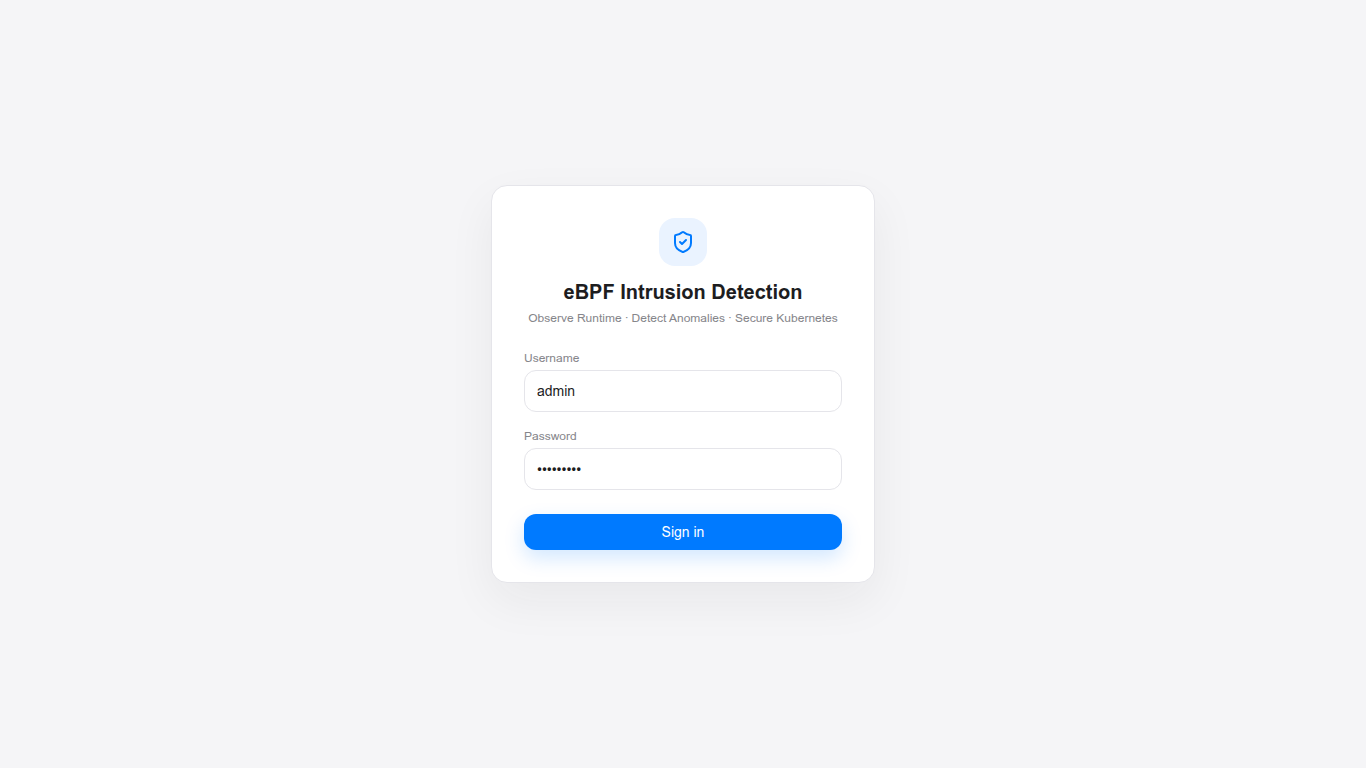
\includegraphics[width=0.82\textwidth]{ss_login.png}
    \caption{Login page}
    \label{fig:ss-login}
\end{figure}

\begin{figure}[H]
    \centering
    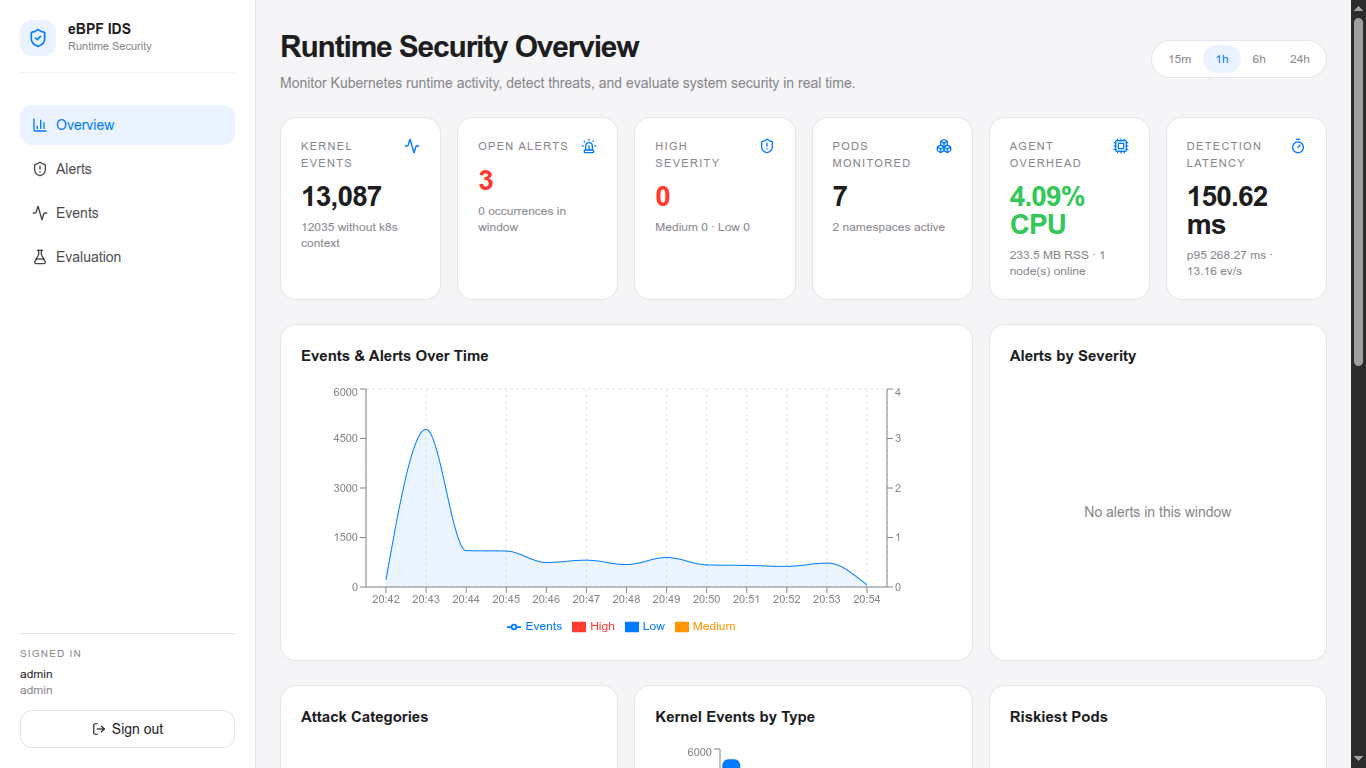
\includegraphics[width=0.95\textwidth]{ss_overview.png}
    \caption{Runtime security overview (top)}
    \label{fig:ss-overview}
\end{figure}

\begin{figure}[H]
    \centering
    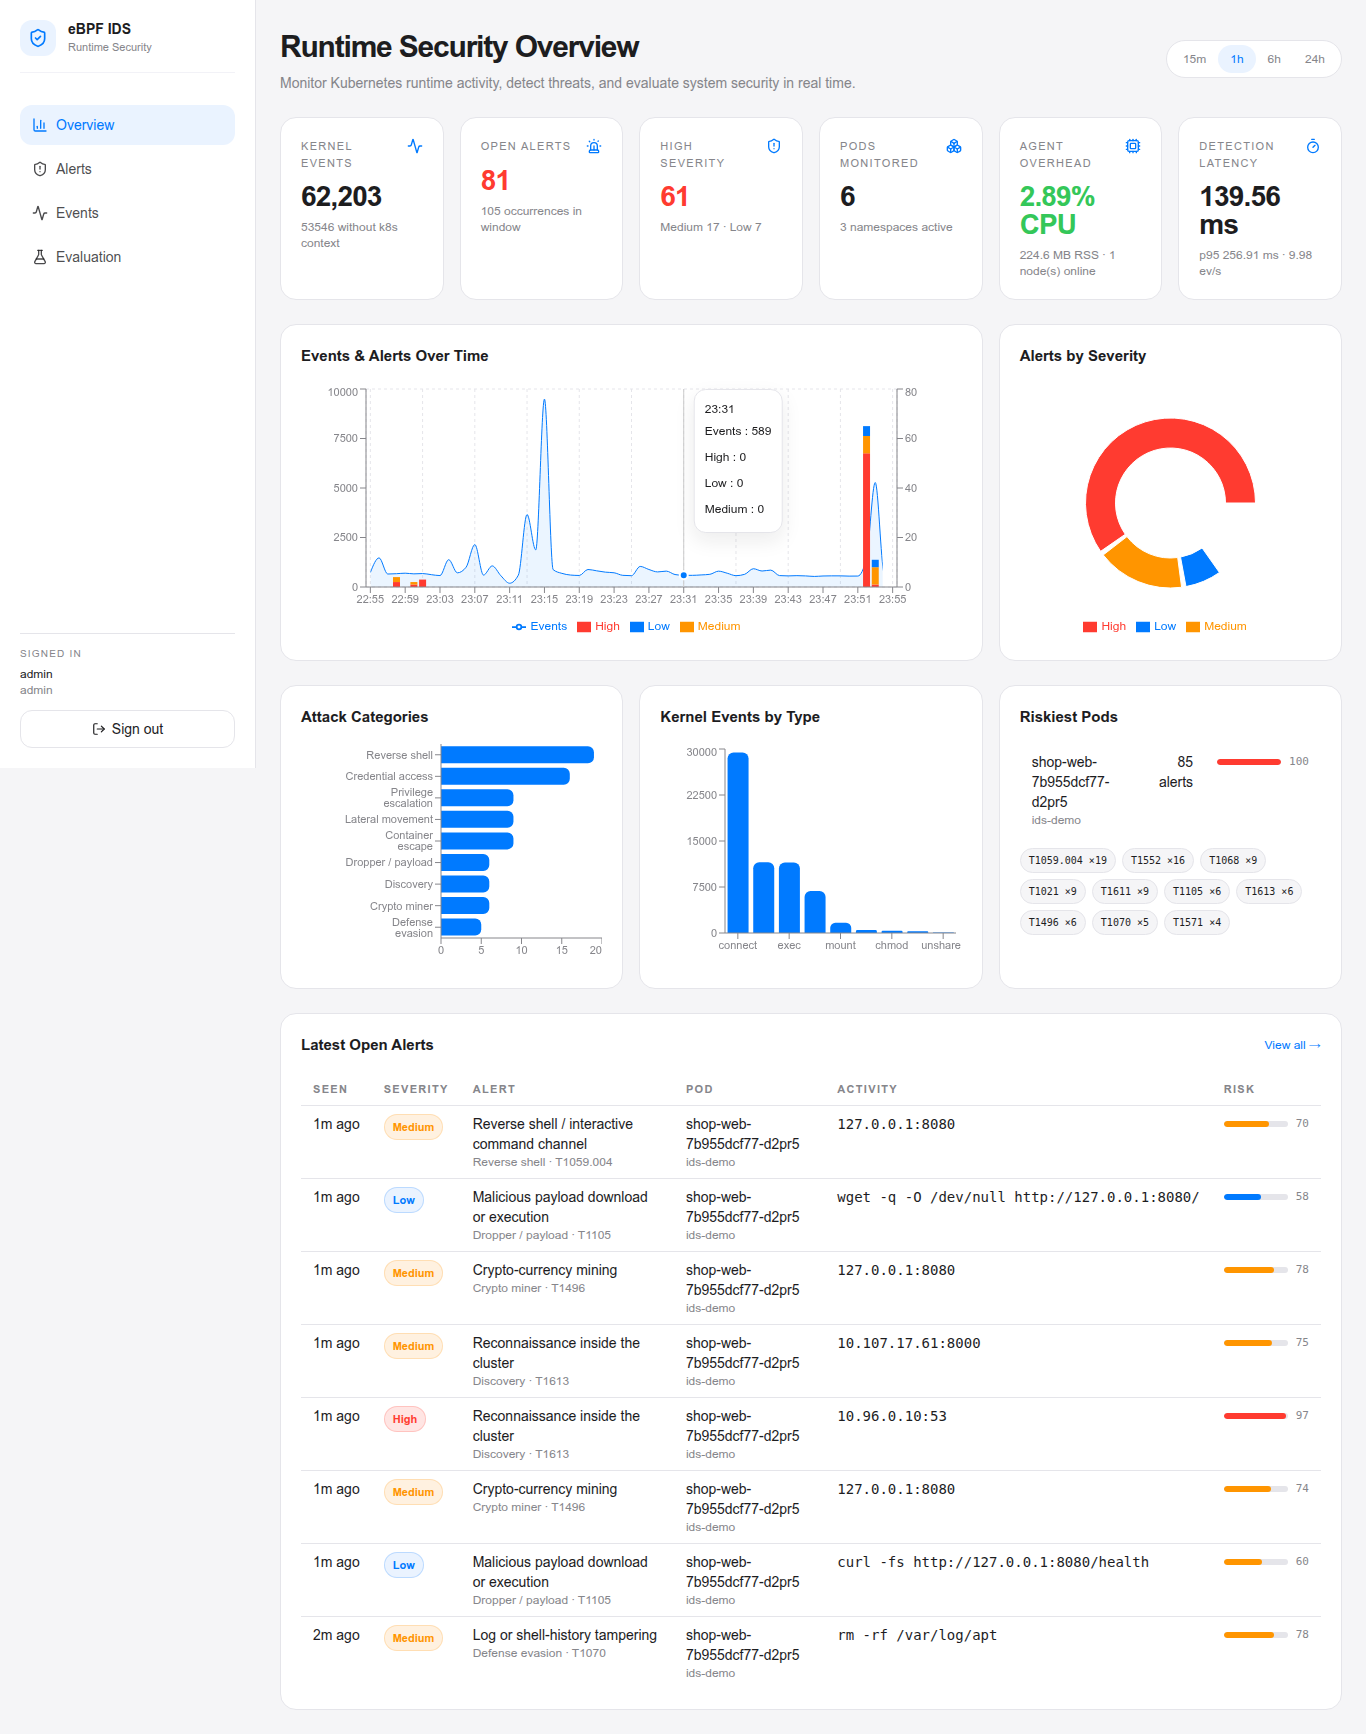
\includegraphics[width=0.8\textwidth]{ss_overview_full.png}
    \caption{Overview after the attack simulation: severities, attack categories,
             kernel event types, riskiest pods with MITRE techniques and latest alerts}
    \label{fig:ss-overview-full}
\end{figure}

\begin{figure}[H]
    \centering
    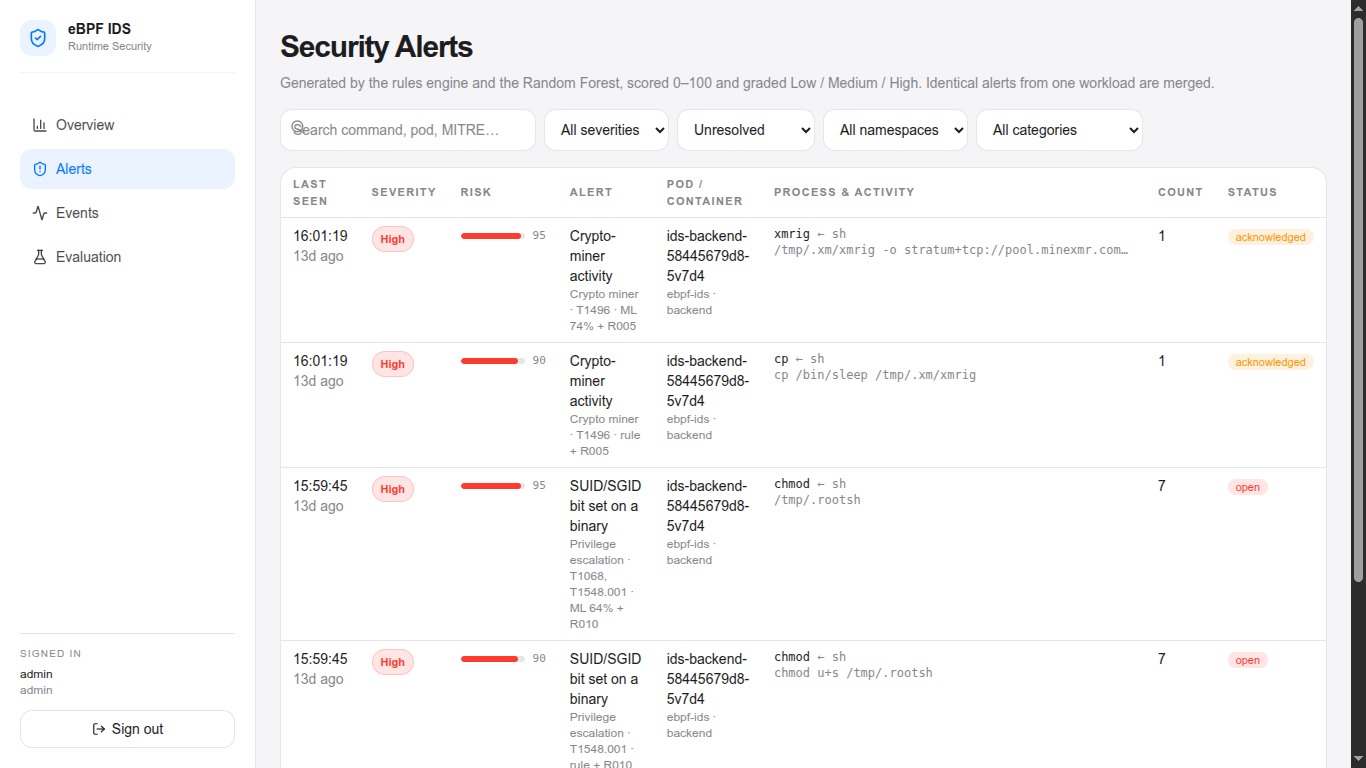
\includegraphics[width=0.95\textwidth]{ss_alerts.png}
    \caption{Security alerts page with risk scores, MITRE techniques and status}
    \label{fig:ss-alerts}
\end{figure}

\begin{figure}[H]
    \centering
    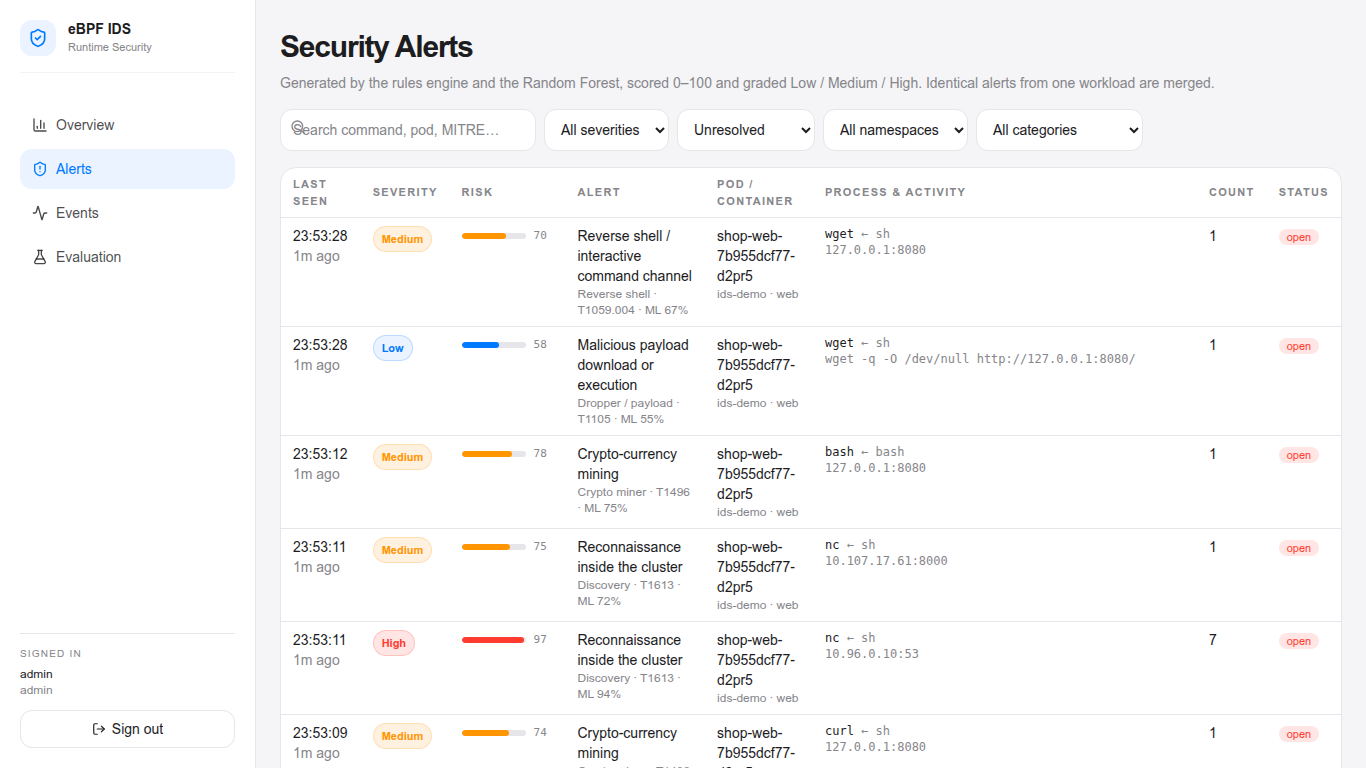
\includegraphics[width=0.95\textwidth]{ss_alerts_live.png}
    \caption{Alerts raised in the test workload \texttt{ids-demo/shop-web}}
    \label{fig:ss-alerts-live}
\end{figure}

\begin{figure}[H]
    \centering
    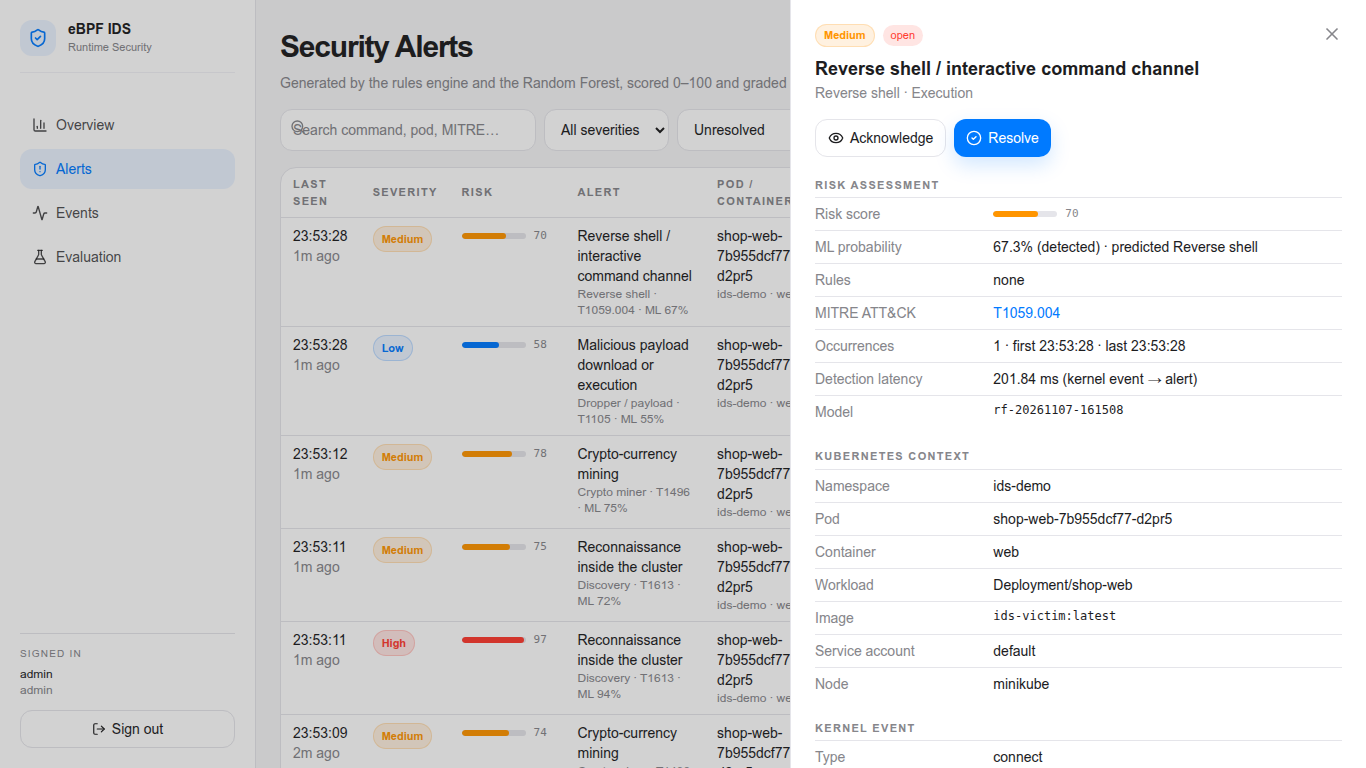
\includegraphics[width=0.95\textwidth]{ss_alert_detail.png}
    \caption{Alert detail panel: risk assessment, ML probability, MITRE technique,
             detection latency and Kubernetes context}
    \label{fig:ss-alert-detail}
\end{figure}

\begin{figure}[H]
    \centering
    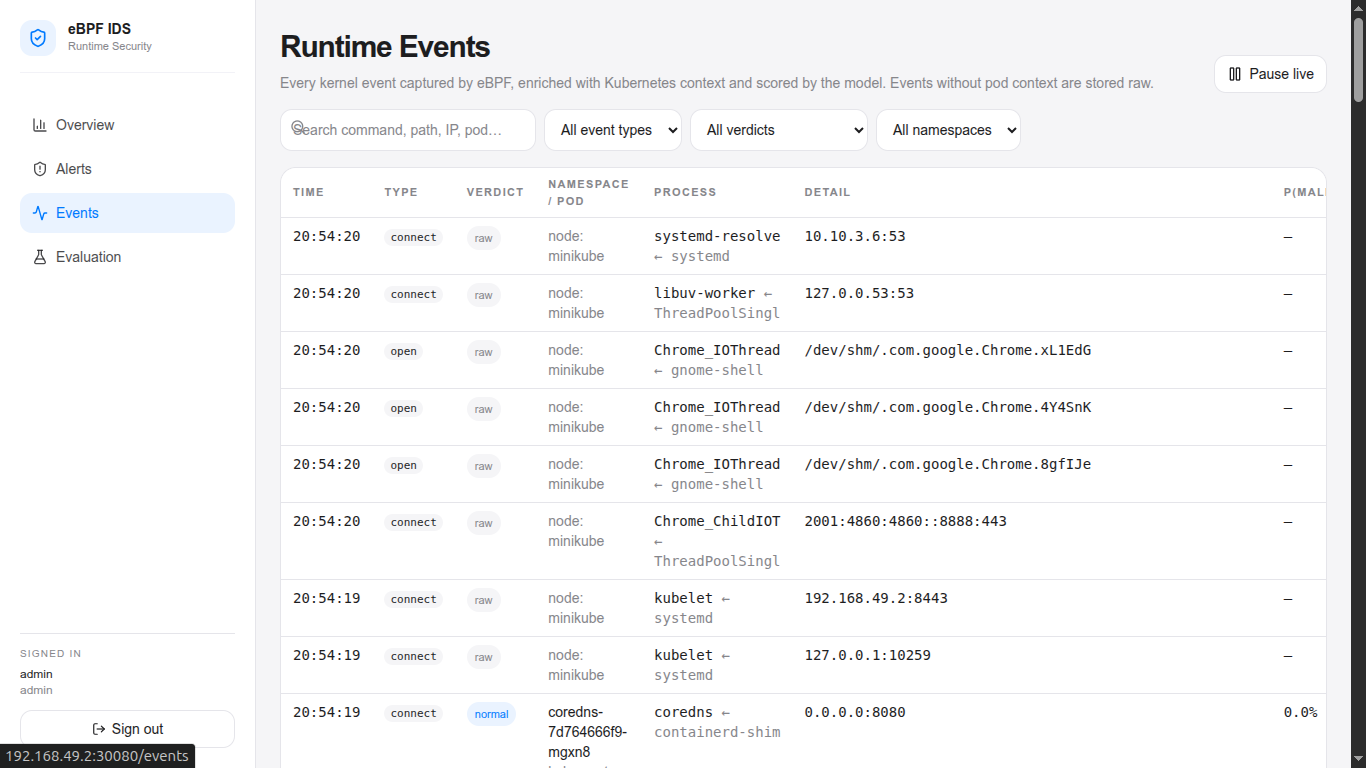
\includegraphics[width=0.95\textwidth]{ss_events.png}
    \caption{Runtime events stream with verdicts}
    \label{fig:ss-events}
\end{figure}

\begin{figure}[H]
    \centering
    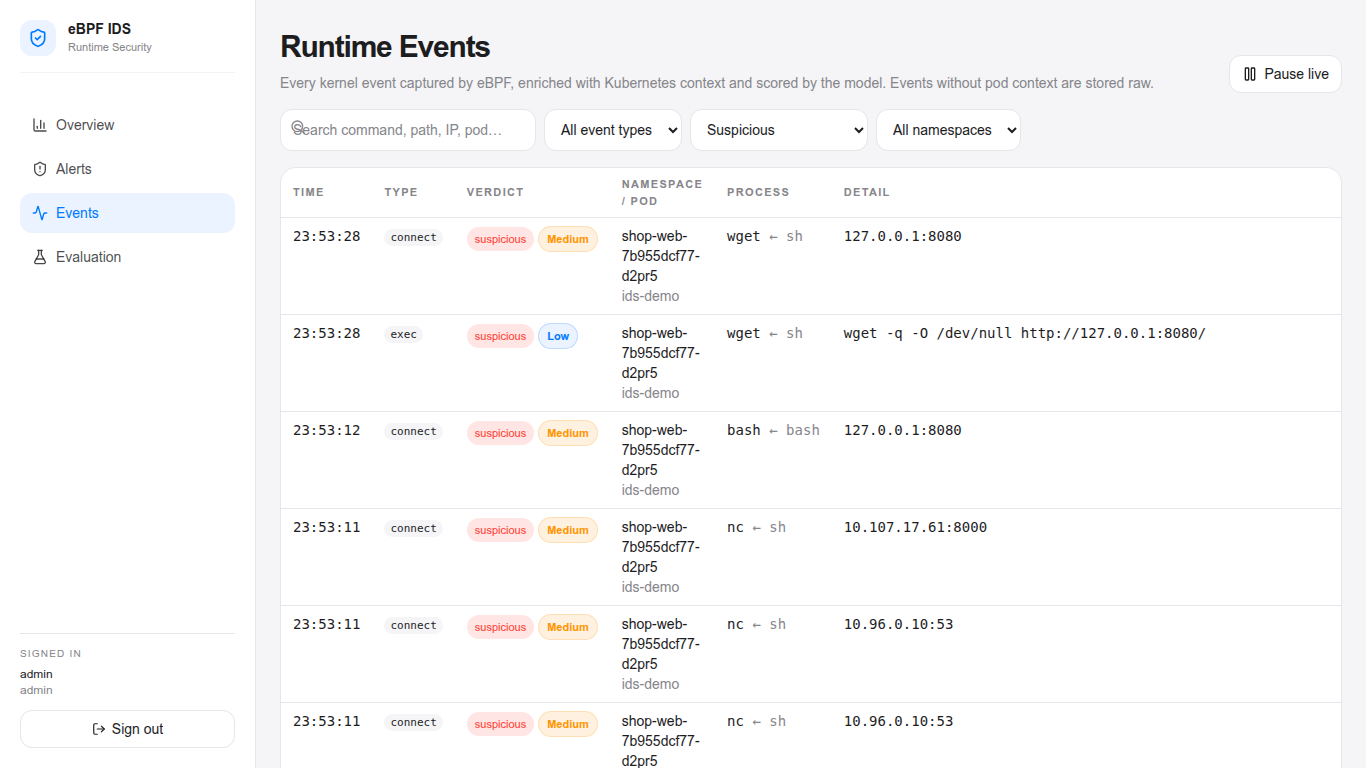
\includegraphics[width=0.95\textwidth]{ss_events_suspicious.png}
    \caption{Events filtered to suspicious verdicts}
    \label{fig:ss-events-sus}
\end{figure}

\begin{figure}[H]
    \centering
    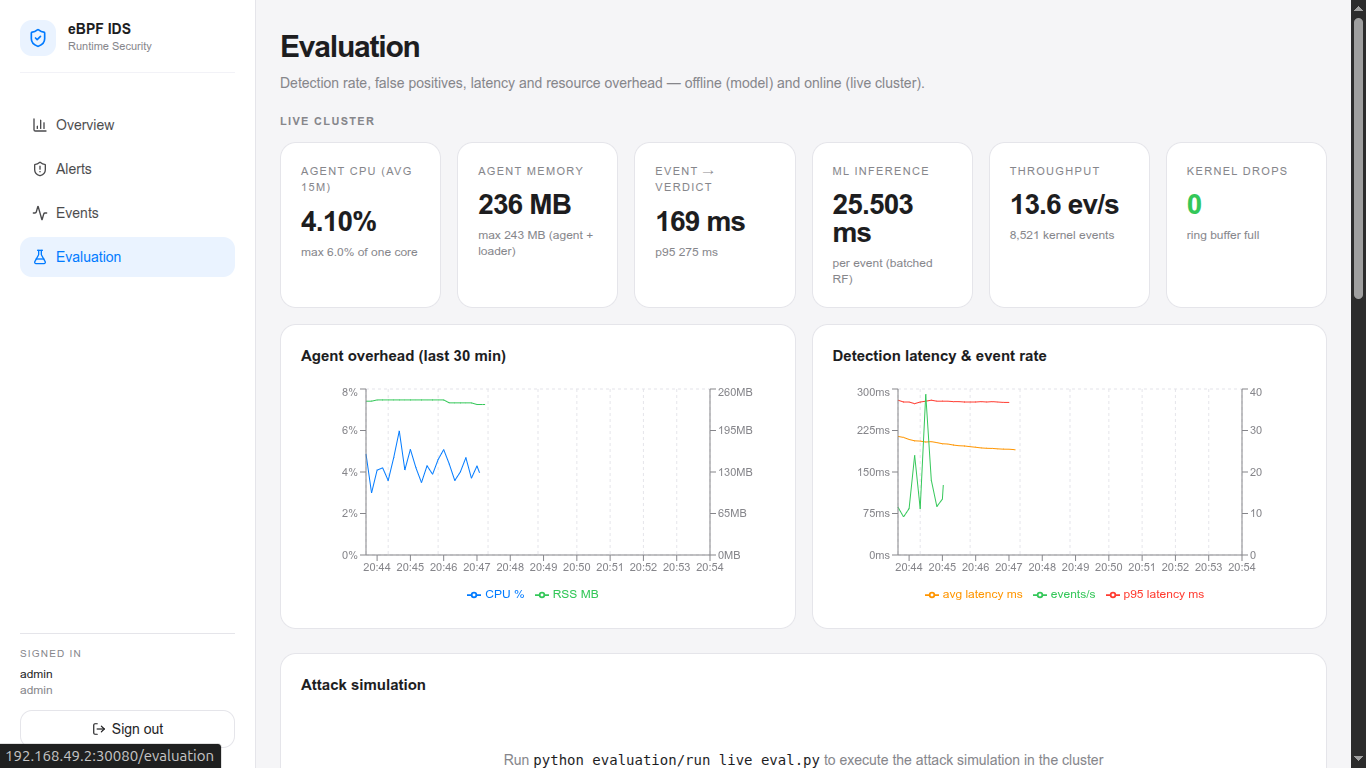
\includegraphics[width=0.95\textwidth]{ss_evaluation_live.png}
    \caption{Evaluation page: live agent overhead, latency and throughput}
    \label{fig:ss-eval-live}
\end{figure}

\begin{figure}[H]
    \centering
    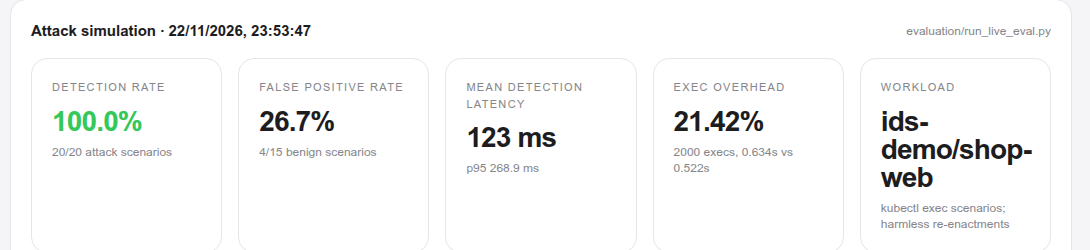
\includegraphics[width=0.95\textwidth]{ss_attack_simulation.png}
    \caption{Evaluation page: attack-simulation summary}
    \label{fig:ss-attack-sim}
\end{figure}

\begin{figure}[H]
    \centering
    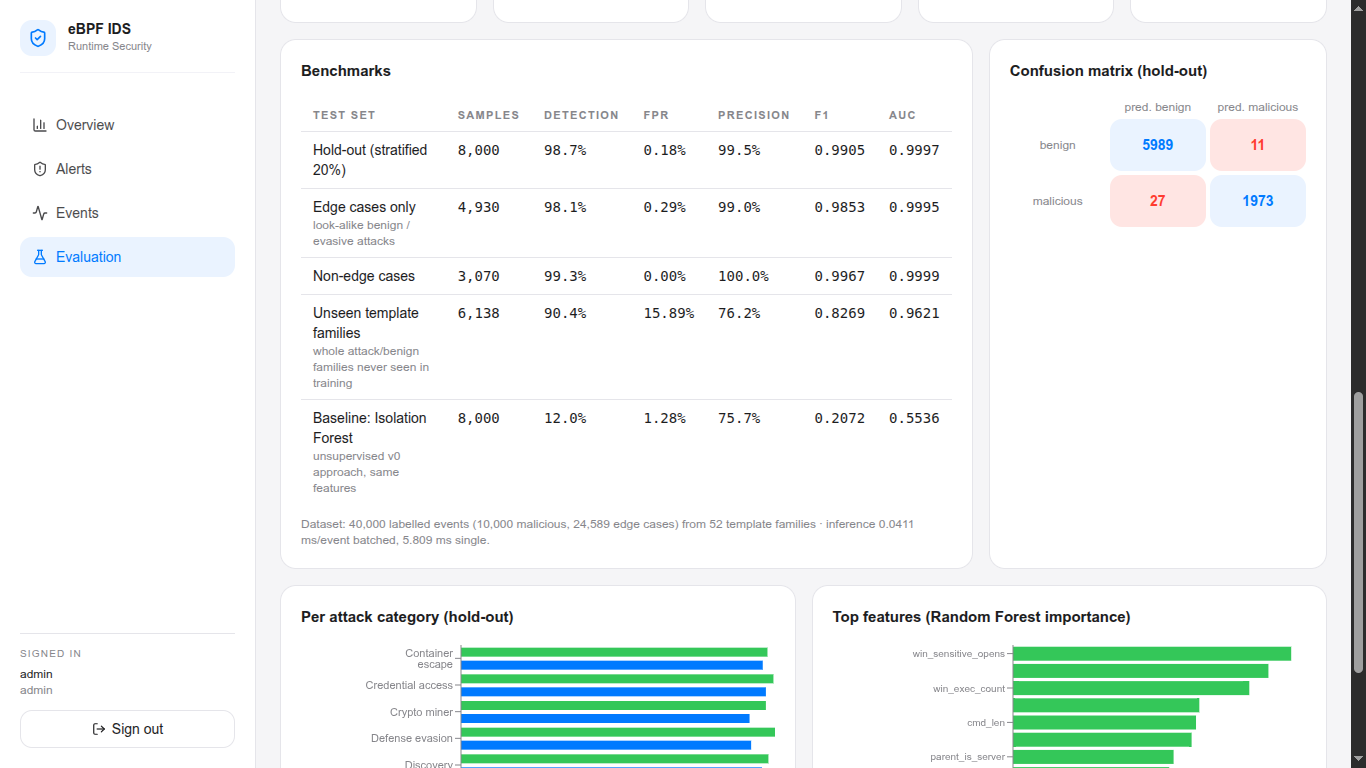
\includegraphics[width=0.95\textwidth]{ss_evaluation_model.png}
    \caption{Evaluation page: offline model benchmarks and confusion matrix}
    \label{fig:ss-eval-model}
\end{figure}

\begin{figure}[H]
    \centering
    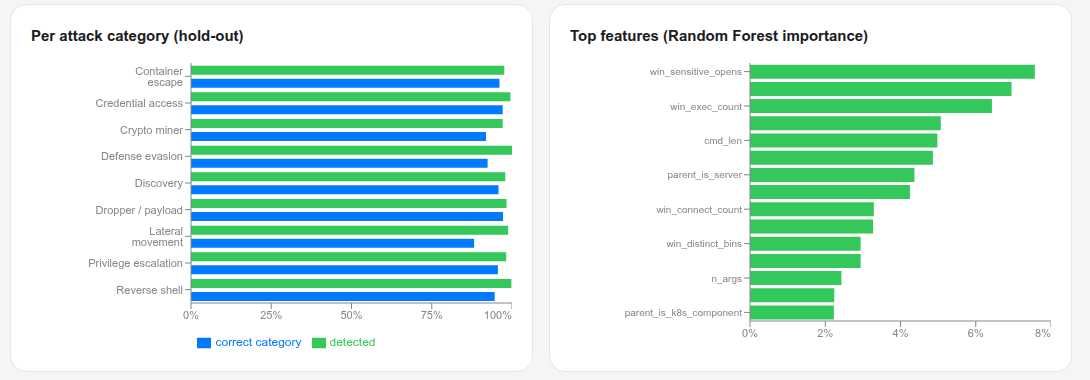
\includegraphics[width=0.95\textwidth]{ss_eval_categories.png}
    \caption{Evaluation page: per-category detection and feature importance}
    \label{fig:ss-eval-cat}
\end{figure}

\chapter{Testing and Results}

Testing was carried out at four levels: unit tests of the agent and backend, user
interface tests of the dashboard, security tests, and an experimental evaluation of
detection quality and performance. The evaluation uses three kinds of data: the
synthetic test set, real-world data (BETH and the Kubernetes escape recording), and a
live attack simulation in the minikube cluster.

\section{Unit Testing}

Unit tests are written with \textbf{pytest}. The backend tests run against a temporary
MongoDB container. All 19 tests pass (Table~\ref{tab:unittests}).

\begin{longtable}{>{\ttfamily\footnotesize}p{6.2cm} >{\raggedright\arraybackslash}p{5.6cm} c}
\caption{Unit tests and results}\label{tab:unittests}\\
\toprule
\normalfont\textbf{Test} & \textbf{What is verified} & \textbf{Result} \\
\midrule
\endfirsthead
\toprule
\normalfont\textbf{Test} & \textbf{What is verified} & \textbf{Result} \\
\midrule
\endhead
\multicolumn{3}{l}{\textit{Agent (services/ebpf-agent/tests) -- 13 tests}} \\
test\_\allowbreak{}normalise\_\allowbreak{}exec\_\allowbreak{}and\_\allowbreak{}connect & Kernel records become pipeline events & Pass \\
test\_\allowbreak{}runc\_\allowbreak{}is\_\allowbreak{}not\_\allowbreak{}netcat & v0 bug: \texttt{runc} no longer matches ``nc'' & Pass \\
test\_\allowbreak{}dev\_\allowbreak{}substring\_\allowbreak{}is\_\allowbreak{}not\_\allowbreak{}suspicious\_\allowbreak{}dir & v0 bug: \texttt{/dev} is not a temp dir & Pass \\
test\_\allowbreak{}features\_\allowbreak{}use\_\allowbreak{}full\_\allowbreak{}argv & Features use all arguments & Pass \\
test\_\allowbreak{}wait\_\allowbreak{}for\_\allowbreak{}is\_\allowbreak{}not\_\allowbreak{}reverse\_\allowbreak{}shell & \texttt{nc -z} wait loops not flagged & Pass \\
test\_\allowbreak{}base64\_\allowbreak{}blob\_\allowbreak{}vs\_\allowbreak{}long\_\allowbreak{}path & Base64 detection vs.\ long paths & Pass \\
test\_\allowbreak{}rules\_\allowbreak{}fire\_\allowbreak{}on\_\allowbreak{}attacks & Rules match attack events & Pass \\
test\_\allowbreak{}rules\_\allowbreak{}quiet\_\allowbreak{}on\_\allowbreak{}platform\_\allowbreak{}behaviour & Platform exemptions work & Pass \\
test\_\allowbreak{}behaviour\_\allowbreak{}tracker\_\allowbreak{}window\_\allowbreak{}and\_\allowbreak{}new\_\allowbreak{}binary & 60 s window and new-binary flag & Pass \\
test\_\allowbreak{}cgroup\_\allowbreak{}regexes\_\allowbreak{}and\_\allowbreak{}workloads & Pod UID, container ID, workload & Pass \\
test\_\allowbreak{}model\_\allowbreak{}separates\_\allowbreak{}attacks\_\allowbreak{}from\_\allowbreak{}benign & Trained model ranks attacks higher & Pass \\
test\_\allowbreak{}assess\_\allowbreak{}produces\_\allowbreak{}alert\_\allowbreak{}with\_\allowbreak{}mitre & Decision has severity and MITRE & Pass \\
test\_\allowbreak{}platform\_\allowbreak{}namespace\_\allowbreak{}needs\_\allowbreak{}high\_\allowbreak{}confidence & 0.75 threshold in platform namespaces & Pass \\
\midrule
\multicolumn{3}{l}{\textit{Backend (services/backend/tests) -- 6 tests}} \\
test\_\allowbreak{}login\_\allowbreak{}rejects\_\allowbreak{}bad\_\allowbreak{}password & Wrong password returns 401 & Pass \\
test\_\allowbreak{}dashboard\_\allowbreak{}requires\_\allowbreak{}jwt & API rejects requests without JWT & Pass \\
test\_\allowbreak{}ingest\_\allowbreak{}requires\_\allowbreak{}agent\_\allowbreak{}token & Ingest rejects missing / wrong token & Pass \\
test\_\allowbreak{}ingest\_\allowbreak{}events\_\allowbreak{}and\_\allowbreak{}dedup\_\allowbreak{}alerts & Events stored, alerts merged & Pass \\
test\_\allowbreak{}alert\_\allowbreak{}lifecycle & Open $\rightarrow$ acknowledged $\rightarrow$ resolved & Pass \\
test\_\allowbreak{}stats\_\allowbreak{}agents\_\allowbreak{}evaluation & Statistics and evaluation endpoints & Pass \\
\bottomrule
\end{longtable}

\section{User Interface Testing}

The dashboard was tested in a real browser with \textbf{Playwright} (Chrome). The test
script logs in with the administrator account, opens every page (Overview, Alerts,
Events, Evaluation), opens an alert's detail panel, applies the ``suspicious'' filter on
the Events page and takes the screenshots shown in Chapter~7. All pages loaded and
displayed live data. The test exposed one layout defect: in the attack-simulation table
of the Evaluation page the result column is too narrow, so only the first rows are
visible without scrolling; this is listed under future work.

\section{Security Testing}

\begin{itemize}
    \item \textbf{Authentication:} dashboard endpoints return 401 without a valid JWT; the
          ingest endpoints reject requests without the agent token (verified by unit tests).
    \item \textbf{Password storage:} the admin password is stored as a bcrypt hash; the
          plain password exists only in the Kubernetes Secret.
    \item \textbf{Secrets:} all credentials are random values generated at deployment, not
          hard-coded in the source code or images.
    \item \textbf{Least privilege:} the agent's ClusterRole allows only reading pods; the
          backend and frontend run without privileges. Only the agent is privileged, which
          is required to load eBPF programs.
    \item \textbf{Robustness:} malformed events and failing rules are skipped without
          stopping the sensor; kernel drops are counted and shown on the dashboard.
\end{itemize}

\section{Evaluation Metrics}

With TP, TN, FP and FN denoting true positives, true negatives, false positives and
false negatives (malicious = positive class), the following metrics are reported:
\begin{align}
\mathrm{Accuracy} &= \frac{TP + TN}{TP + TN + FP + FN} \\
\mathrm{Precision} &= \frac{TP}{TP + FP} \\
\mathrm{Recall\ (detection\ rate)} &= \frac{TP}{TP + FN} \\
\mathrm{FPR} &= \frac{FP}{FP + TN} \\
F_1 &= 2 \cdot \frac{\mathrm{Precision} \cdot \mathrm{Recall}}{\mathrm{Precision} + \mathrm{Recall}}
\end{align}
ROC-AUC is the area under the curve of recall against FPR over all thresholds; it
measures how well the model \emph{ranks} malicious events above benign ones,
independently of the chosen threshold. For an IDS the false-positive rate matters as
much as recall: on a busy node even 1\% false positives produce many alerts per hour.

\section{Results on the Synthetic Data (Deployed Model)}

The model deployed in the cluster (\texttt{rf-20261107-161508}) was trained on the
40,000-row synthetic dataset. Table~\ref{tab:offline} shows its results on a stratified
20\% hold-out and on harder subsets, compared with the Isolation Forest baseline of the
v0 prototype; Figure~\ref{fig:cm-holdout} shows the hold-out confusion matrix.

\begin{table}[H]
\centering
\caption{Offline results of the deployed model (synthetic data, threshold 0.5)}
\label{tab:offline}
\small
\begin{tabular}{lrrrrrr}
\toprule
\textbf{Test set} & \textbf{Samples} & \textbf{Recall} & \textbf{FPR} & \textbf{Precision} & \textbf{F1} & \textbf{AUC} \\
\midrule
Hold-out (stratified 20\%) & 8,000 & 98.7\% & 0.18\% & 99.5\% & 0.9905 & 0.9997 \\
Edge cases only            & 4,930 & 98.1\% & 0.29\% & 99.0\% & 0.9853 & 0.9995 \\
Non-edge cases             & 3,070 & 99.3\% & 0.00\% & 100.0\% & 0.9967 & 0.9999 \\
Unseen template families   & 6,138 & 90.4\% & 15.89\% & 76.2\% & 0.8269 & 0.9621 \\
\midrule
Baseline: Isolation Forest & 8,000 & 12.0\% & 1.28\% & 75.7\% & 0.2072 & 0.5536 \\
\bottomrule
\end{tabular}
\end{table}

\begin{figure}[H]
\centering
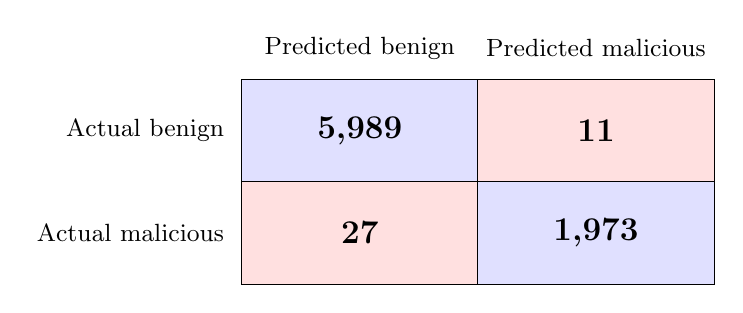
\begin{tikzpicture}[cell/.style={draw, minimum width=3cm, minimum height=1.3cm, font=\large\bfseries}]
  \node[cell, fill=blue!12] at (0,0) {5,989};
  \node[cell, fill=red!12] at (3,0) {11};
  \node[cell, fill=red!12] at (0,-1.3) {27};
  \node[cell, fill=blue!12] at (3,-1.3) {1,973};
  \node[font=\small] at (0,1.05) {Predicted benign};
  \node[font=\small] at (3,1.05) {Predicted malicious};
  \node[font=\small, anchor=east] at (-1.6,0) {Actual benign};
  \node[font=\small, anchor=east] at (-1.6,-1.3) {Actual malicious};
\end{tikzpicture}
\caption{Confusion matrix of the deployed model on the synthetic hold-out set}
\label{fig:cm-holdout}
\end{figure}

\textbf{Observations.} Accuracy on the hold-out set is 99.52\% and five-fold
cross-validation gives $F_1 = 0.9903 \pm 0.0006$. The Random Forest detects eight
times more attacks than the Isolation Forest baseline at a lower false-positive rate.
The ``unseen template families'' row trains without whole families of commands and
tests on them; its recall of 90.4\% at 15.9\% FPR is the more realistic estimate of
generalisation, and closing this gap is the job of the rule layer. The most important
features are the behaviour-window counters (sensitive opens, shell count, execution
count, new binary), command-line length and entropy, and whether the parent is a
server process. Inference takes 0.04~ms per event in batches of 256.

\section{Results on the Final Test Set}

A second model (\texttt{rf-20261122-223113}) was trained with exactly the same method
on the final \texttt{train.csv} (synthetic data plus 25,000 real benign BETH events) and
tested once on \texttt{test.csv} (Section~4.5). No parameter or threshold was tuned on
the test set.

\subsection{Validation on the Training Data}

\begin{table}[H]
\centering
\caption{Validation of the final model on \texttt{train.csv}}
\label{tab:finalval}
\small
\begin{tabular}{lrrrrr}
\toprule
\textbf{Check} & \textbf{Accuracy} & \textbf{Precision} & \textbf{Recall} & \textbf{FPR} & \textbf{F1} \\
\midrule
Stratified 20\% hold-out (13,000)   & 0.9975 & 0.9945 & 0.9895 & 0.10\% & 0.9920 \\
Edge cases only (4,906)             & 0.9945 & 0.9906 & 0.9842 & 0.26\% & 0.9874 \\
Unseen template families (7,711)    & 0.9684 & 0.9894 & 0.9105 & 0.46\% & 0.9483 \\
5-fold cross-validation             & --     & --     & 0.9877 & 0.10\% & 0.9912 \\
Baseline: Isolation Forest          & 0.8679 & 0.7737 & 0.2000 & 1.06\% & 0.3178 \\
\bottomrule
\end{tabular}
\end{table}

Adding real benign data reduced the false-positive rate on unseen template families
from 15.89\% to 0.46\%.

\subsection{Binary Results per Test Source}

\begin{table}[H]
\centering
\caption{Final model on \texttt{test.csv} (ML only, threshold 0.5)}
\label{tab:finaltest}
\scriptsize
\setlength{\tabcolsep}{3pt}
\begin{tabular}{lrrrrrrrrrr}
\toprule
\textbf{Source} & \textbf{Samples} & \textbf{Acc.} & \textbf{Prec.} & \textbf{Recall} & \textbf{FPR} & \textbf{F1} & \textbf{AUC} & \textbf{FP} & \textbf{FN} & \textbf{TP} \\
\midrule
Synthetic        & 20,000  & 0.9939 & 0.9986 & 0.9860 & 0.09\% & \textbf{0.9923} & 0.9998 & 11 & 112 & 7,888 \\
BETH (real)      & 262,825 & 0.4427 & 0.9988 & 0.0056 & 0.00\% & \textbf{0.0112} & 0.9995 & 1 & 146,479 & 829 \\
K8s escape       & 25      & 0.7200 & 0.5000 & 0.1429 & 5.56\% & \textbf{0.2222} & 0.6746 & 1 & 6 & 1 \\
\midrule
All (ML only)    & 282,850 & 0.4817 & 0.9985 & 0.0561 & 0.01\% & 0.1063 & 0.9991 & 13 & 146,597 & 8,718 \\
All (ML + rules) & 282,850 & 0.4794 & 0.9230 & 0.0566 & 0.57\% & 0.1066 & -- & 733 & 146,527 & 8,788 \\
\bottomrule
\end{tabular}
\end{table}

\begin{figure}[H]
\centering
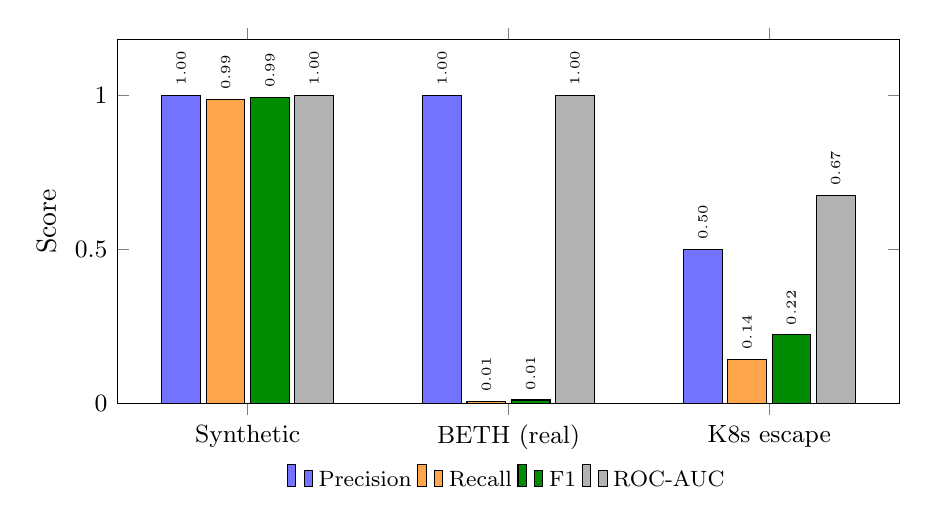
\begin{tikzpicture}
\begin{axis}[
    ybar, bar width=14pt, width=0.95\textwidth, height=6.2cm,
    ymin=0, ymax=1.18, ylabel={Score},
    symbolic x coords={Synthetic, BETH (real), K8s escape},
    xtick=data, enlarge x limits=0.25,
    legend style={at={(0.5,-0.15)}, anchor=north, legend columns=-1, font=\footnotesize, draw=none},
    nodes near coords, nodes near coords style={/pgf/number format/fixed, /pgf/number format/fixed zerofill, /pgf/number format/precision=2},
    every node near coord/.append style={font=\tiny, rotate=90, anchor=west},
    tick label style={font=\small}]
  \addplot[fill=blue!55] coordinates {(Synthetic,0.9986) (BETH (real),0.9988) (K8s escape,0.5)};
  \addplot[fill=orange!70] coordinates {(Synthetic,0.986) (BETH (real),0.0056) (K8s escape,0.1429)};
  \addplot[fill=green!55!black] coordinates {(Synthetic,0.9923) (BETH (real),0.0112) (K8s escape,0.2222)};
  \addplot[fill=gray!60] coordinates {(Synthetic,0.9998) (BETH (real),0.9995) (K8s escape,0.6746)};
  \legend{Precision, Recall, F1, ROC-AUC}
\end{axis}
\end{tikzpicture}
\caption{Precision, recall, F1 and ROC-AUC of the final model per test source}
\label{fig:persource}
\end{figure}

\subsection{Multi-Class Results}

On all test rows whose true category is known (synthetic, Kubernetes escape and BETH
benign events), the model reaches a multi-class accuracy of 99.68\%, a macro-averaged
F1 of 0.9554 and a weighted F1 of 0.9968 (Table~\ref{tab:multiclass}).

\begin{table}[H]
\centering
\caption{Per-class results of the final model on \texttt{test.csv}}
\label{tab:multiclass}
\small
\begin{tabular}{lrrrr}
\toprule
\textbf{Class} & \textbf{Precision} & \textbf{Recall} & \textbf{F1} & \textbf{Support} \\
\midrule
Benign               & 0.9981 & 1.0000 & 0.9991 & 127,535 \\
Container escape     & 0.9975 & 0.9736 & 0.9854 & 833 \\
Credential access    & 0.9987 & 0.9544 & 0.9761 & 812 \\
Crypto-miner         & 0.9972 & 0.9273 & 0.9610 & 757 \\
Defense evasion      & 0.9983 & 0.9190 & 0.9570 & 630 \\
Discovery            & 0.9344 & 0.9712 & 0.9525 & 939 \\
Dropper / payload    & 0.9701 & 0.9719 & 0.9710 & 1,102 \\
Lateral movement     & 0.9590 & 0.7524 & 0.8432 & 311 \\
Privilege escalation & 0.9205 & 0.9399 & 0.9301 & 949 \\
Reverse shell        & 0.9994 & 0.9582 & 0.9783 & 1,674 \\
\midrule
Macro average        & 0.9773 & 0.9368 & 0.9554 & \\
\bottomrule
\end{tabular}
\end{table}

The weakest class is lateral movement, which is often confused with discovery (54 of
311 events) because both consist of connections to internal services.

\subsection{Comparison with the Deployed Model}

\begin{table}[H]
\centering
\caption{Deployed model vs.\ final model on \texttt{test.csv} (ML only, threshold 0.5)}
\label{tab:compare}
\small
\begin{tabular}{lcc}
\toprule
\textbf{Test source} & \textbf{Deployed model} & \textbf{Final model} \\
 & F1 / Recall / FP & F1 / Recall / FP \\
\midrule
Synthetic          & 0.9921 / 0.9862 / 15  & 0.9923 / 0.9860 / 11 \\
BETH (real)        & 0.6869 / 0.5248 / 481 & 0.0112 / 0.0056 / 1 \\
Kubernetes escape  & 0.2222 / 0.1429 / 1   & 0.2222 / 0.1429 / 1 \\
\bottomrule
\end{tabular}
\end{table}

\subsection{Analysis of the Real-World Results}

\begin{itemize}
    \item \textbf{False positives almost eliminated.} Real benign host activity in the
          training data (\texttt{ps} reading \texttt{/proc}, \texttt{sshd}, systemd) cut
          the false positives on the BETH test hosts from 481 to 1.
    \item \textbf{Recall on BETH collapsed at the 0.5 threshold.} 144,801 of the 147,308
          malicious BETH events come from one SSH-scanning bot. Benign \texttt{sshd}
          connections to port 22 in the new training data lowered the scanner's score to
          about 0.47, just below the threshold. The ranking is still excellent (ROC-AUC
          0.9995): the scanner is scored above almost all benign events, but not above
          0.5. The root cause is a training gap: no synthetic attack contains more than 12
          distinct destinations in its window, whereas the scanner contacts about 3,200.
    \item \textbf{Threshold.} At thresholds of 0.2--0.3 the F1 on the whole test set would
          exceed 0.99. This was deliberately \emph{not} used, because choosing the
          threshold on the test set would make the test result meaningless, and the
          improvement is caused by a single cluster of scanner events.
    \item \textbf{Other BETH attacks} (about 2,500 events) are partly label noise (BETH
          labels routine commands of the attacker's session as evil) and partly real
          misses, such as \texttt{wget} from a raw IP address (score 0.49) and
          \texttt{modprobe msr} (0.29).
    \item \textbf{Kubernetes escape.} Only the \texttt{nsenter --target 1} step is flagged
          (rule R014 and ML); the follow-up actions are missed. The recording contains only
          process executions, whereas the live sensor would also observe the
          \texttt{open} of \texttt{/root/.ssh/authorized\_keys} and the \texttt{mount}
          system call, which the rules target. The incident as a whole is detected.
\end{itemize}
These results confirm the observation of Sommer and Paxson~\cite{sommer2010}: excellent
in-distribution results do not guarantee real-world performance. For this reason the
deployed model was \emph{not} replaced by the final model.

\section{Live Cluster Evaluation}

The script \texttt{evaluation/run\_live\_eval.py} runs 20 harmless attack re-enactments
and 15 benign look-alike commands with \texttt{kubectl exec} inside the test workload
\texttt{ids-demo/shop-web} and checks which of them produce an alert. It then measures
execution overhead by running 2,000 fork+exec operations with and without the agent.
Table~\ref{tab:live} summarises the run of 22 November 2026; Table~\ref{tab:scenarios}
lists every scenario.

\begin{table}[H]
\centering
\caption{Live evaluation in minikube}
\label{tab:live}
\small
\begin{tabular}{ll}
\toprule
\textbf{Metric} & \textbf{Result} \\
\midrule
Attack scenarios detected & \textbf{20 / 20 (100\%)} \\
Benign scenarios flagged (false positives) & 4 / 15 (26.7\%) \\
Detection latency (kernel event $\rightarrow$ verdict) & average \textbf{123 ms}, p95 269 ms \\
Kernel events dropped & 0 \\
Agent CPU (normal load) & 3.5\% of one core \\
Agent memory & 198 MB (agent 189 MB + loader 9 MB) \\
Event throughput during the run & 23.5 events/s \\
Execution overhead (2,000 $\times$ fork+exec) & +21.4\% (0.634 s vs.\ 0.522 s) \\
\bottomrule
\end{tabular}
\end{table}

{\small
\begin{longtable}{>{\raggedright\arraybackslash}p{4.4cm} l l l >{\raggedright\arraybackslash}p{3.2cm}}
\caption{Live attack and benign scenarios}\label{tab:scenarios}\\
\toprule
\textbf{Scenario} & \textbf{Kind} & \textbf{Result} & \textbf{Sev.} & \textbf{Latency / rules} \\
\midrule
\endfirsthead
\toprule
\textbf{Scenario} & \textbf{Kind} & \textbf{Result} & \textbf{Sev.} & \textbf{Latency / rules} \\
\midrule
\endhead
Bash reverse shell & attack & detected & High & 109 ms, R001, R002 \\
Netcat reverse shell & attack & detected & High & 177 ms, R001, R002 \\
Python reverse shell & attack & detected & High & 32 ms, R001, R002 \\
Download piped to shell & attack & detected & High & 58 ms, R006 \\
Hidden binary run from /tmp & attack & detected & High & 215 ms, R007 \\
Crypto-miner process & attack & detected & High & 210 ms, R005 \\
Miner connecting to pool & attack & detected & High & 25 ms, R005, R007 \\
Service-account token theft & attack & detected & High & 150 ms, R003 \\
Password database read & attack & detected & High & 37 ms, R004 \\
Cloud metadata query & attack & detected & High & 152 ms, R015 \\
SUID shell backdoor & attack & detected & High & 36 ms, R010 \\
Cron persistence & attack & detected & High & 155 ms, R006, R016 \\
nsenter into host namespaces & attack & detected & High & 29 ms, R014 \\
User-namespace unshare & attack & detected & High & 140 ms, R014 \\
Docker socket access & attack & detected & High & 269 ms, R014 \\
Kubelet API access & attack & detected & High & 131 ms, R017 \\
Internal port scan & attack & detected & High & 36 ms, R018 \\
Container recon & attack & detected & Low & 235 ms, ML only \\
Fileless memfd payload & attack & detected & High & 73 ms, R012 \\
History / log wiping & attack & detected & Medium & 191 ms, R013 \\
\midrule
List application files & benign & clean & -- & -- \\
Read hostname & benign & clean & -- & -- \\
Python one-liner & benign & clean & -- & -- \\
Local health check (curl) & benign & false positive & Medium & ML only \\
Wait-for dependency (nc -z) & benign & false positive & Medium & ML only \\
Port check via /dev/tcp & benign & false positive & Medium & ML only \\
Process listing & benign & clean & -- & -- \\
Decode base64 config & benign & clean & -- & -- \\
pip version & benign & clean & -- & -- \\
Find python files & benign & clean & -- & -- \\
Backup app directory & benign & clean & -- & -- \\
Pretty-print JSON config & benign & clean & -- & -- \\
Check environment variable & benign & clean & -- & -- \\
Disk usage & benign & clean & -- & -- \\
Fetch own API (wget) & benign & false positive & Medium & ML only \\
\bottomrule
\end{longtable}
}

\textbf{Observations.} Every attack was detected, 18 of 20 with High severity and
most of them by both a rule and the model. All four false positives are ML-only
verdicts for network checks (\texttt{curl}, \texttt{nc -z}, \texttt{/dev/tcp},
\texttt{wget} to localhost) typed in an interactive \texttt{kubectl exec} shell, which
the model associates with attacker sessions; no rule fired for them. The same checks
run from an entrypoint or a probe look different in the behaviour window and are not
flagged in the training data. Detection latency is well below one second, no kernel
events were lost and the agent's CPU and memory use are small. The execution overhead
of 21\% is a worst-case micro-benchmark in which every one of 2,000 back-to-back
executions is captured and scored in Python; at the normal event rate of a few events
per second the overhead is negligible.

\section{Summary of Results}

\begin{itemize}
    \item On synthetic data the model reaches \textbf{F1 = 0.992} with a false-positive
          rate below 0.2\%, eight times the detection rate of the Isolation Forest
          baseline.
    \item In the live cluster the complete system (eBPF sensor, ML and rules) detected
          \textbf{20 of 20 attacks} with an average latency of \textbf{123 ms}, 3.5\% CPU
          and about 200 MB of memory.
    \item On real-world data precision stays very high, but recall shows that the
          synthetic attack examples do not cover real attacker behaviour such as mass SSH
          scanning; improving the training data is the most important next step.
\end{itemize}

\chapter{Conclusion and Future Scope}

\section{Conclusion}

This project designed, implemented and evaluated an \textbf{eBPF-based runtime
intrusion detection system for Kubernetes}. The system observes the kernel activity of
every container through an eBPF program on 16 system-call tracepoints, attaches Pod,
container, namespace and workload identity to each event, extracts 74 behavioural
features and classifies them with a 10-class Random Forest combined with 19
deterministic rules. Every suspicious event becomes an explainable alert with a 0--100
risk score, a Low / Medium / High severity and a MITRE ATT\&CK technique, which is
stored in MongoDB, served by a FastAPI backend and visualised in a React dashboard. The
whole system is deployed on minikube with a single script.

The main outcomes are:
\begin{itemize}
    \item A working end-to-end pipeline \emph{Observe $\rightarrow$ Enrich $\rightarrow$
          Detect $\rightarrow$ Score $\rightarrow$ Alert $\rightarrow$ Evaluate} that runs as
          a standard Kubernetes DaemonSet without changes to the monitored applications.
    \item A labelled runtime-telemetry dataset of 52 template families with deliberate
          edge cases, and converters that map the public BETH dataset and Tetragon
          recordings to the same schema.
    \item A model that reaches an F1-score of 0.992 with a false-positive rate below
          0.2\% on held-out synthetic data and detects eight times more attacks than the
          Isolation Forest baseline of the first prototype.
    \item Detection of \textbf{all 20 attack re-enactments} in the live cluster with an
          average latency of \textbf{123 ms}, about 3.5\% of one CPU core, 200 MB of
          memory and no lost kernel events.
    \item An honest evaluation on real-world data, which showed very high precision but
          also that synthetic attack examples do not cover all real attacker behaviour.
\end{itemize}

The project demonstrates that eBPF makes kernel-level runtime visibility practical in
Kubernetes, and that combining interpretable rules with machine learning gives
detections that are both broad and explainable. Its evaluation also shows why
intrusion-detection results must be measured on data that differs from the training
data before a model is trusted in production.

\section{Limitations}

\begin{itemize}
    \item \textbf{Synthetic attack data:} all attack examples used for training are
          generated; real-world recall is much lower than in-distribution recall
          (Section~8.6).
    \item \textbf{False positives from interactive shells:} network checks typed in an
          interactive \texttt{kubectl exec} shell are flagged by the model.
    \item \textbf{File paths:} file monitoring matches absolute paths only; relative
          \texttt{openat} paths (for example after \texttt{cd /etc}) are not resolved.
    \item \textbf{Argument truncation:} arguments are limited to 8 $\times$ 127 bytes in the
          kernel.
    \item \textbf{Overhead under exec storms:} every execution is scored in Python, which
          costs about 21\% extra time in an exec-heavy micro-benchmark.
    \item \textbf{Detection only:} the system raises alerts but does not block or kill
          malicious processes.
    \item \textbf{Scale:} the system was evaluated on a single-node minikube cluster.
\end{itemize}

\section{Future Scope}

\begin{itemize}
    \item \textbf{Better training data:} add generic attack families revealed by the
          real-world evaluation (mass network scanning and worm spreading, downloads from
          raw IP addresses, miners in hidden temporary directories, miner tuning such as
          \texttt{modprobe msr}) and collect labelled telemetry from real workloads, while
          keeping the BETH test hosts strictly for testing.
    \item \textbf{Threshold calibration} on a validation split of the training data
          instead of a fixed 0.5.
    \item \textbf{Sequence and graph models:} model the order of events in a session or the
          process tree (for example with recurrent networks or graph neural networks) to
          catch multi-step attacks that look harmless event by event.
    \item \textbf{Prevention:} use eBPF LSM hooks or Tetragon-style enforcement to block
          high-confidence attacks such as container escapes in the kernel.
    \item \textbf{Lower overhead:} move more filtering into the kernel, score only events
          with Kubernetes context, and replace the Python window computation with an
          incremental implementation (already used in the dataset converter).
    \item \textbf{Multi-node and cloud deployment:} evaluate on multi-node clusters with
          higher event rates and on managed Kubernetes services.
    \item \textbf{Integrations:} send alerts to Slack, e-mail or a SIEM, and export metrics
          to Prometheus and Grafana.
    \item \textbf{Dashboard:} fix the narrow result column of the attack-simulation table,
          add role-based users and alert assignment.
\end{itemize}

With these improvements the system can grow from a working research prototype into a
practical runtime-security tool for small and medium-sized organisations that run
their applications on Kubernetes.


\clearpage
\renewcommand{\bibname}{References}
\phantomsection
\addcontentsline{toc}{chapter}{References}
\begin{thebibliography}{99}

\bibitem{forrest1996}
S.~Forrest, S.~A.~Hofmeyr, A.~Somayaji and T.~A.~Longstaff, ``A sense of self for Unix
processes,'' in \textit{Proc. IEEE Symposium on Security and Privacy}, 1996, pp.~120--128.

\bibitem{creech2013}
G.~Creech and J.~Hu, ``Generation of a new IDS test dataset: Time to retire the KDD
collection,'' in \textit{Proc. IEEE Wireless Communications and Networking Conference
(WCNC)}, 2013, pp.~4487--4492.

\bibitem{sultan2019}
S.~Sultan, I.~Ahmad and T.~Dimitriou, ``Container security: Issues, challenges, and the
road ahead,'' \textit{IEEE Access}, vol.~7, pp.~52976--52996, 2019.

\bibitem{mitre}
MITRE Corporation, \textit{MITRE ATT\&CK -- Containers Matrix}. Available at:
\url{https://attack.mitre.org/matrices/enterprise/containers/}

\bibitem{abed2015}
A.~S.~Abed, C.~Clancy and D.~S.~Levy, ``Applying bag of system calls for anomalous
behavior detection of applications in Linux containers,'' in \textit{Proc. IEEE
Globecom Workshops}, 2015.

\bibitem{tien2019}
C.-W.~Tien, T.-Y.~Huang, C.-W.~Tien, T.-C.~Huang and S.-Y.~Kuo, ``KubAnomaly: Anomaly
detection for the Docker orchestration platform with neural network approaches,''
\textit{Engineering Reports}, vol.~1, no.~5, 2019.

\bibitem{karn2021}
R.~R.~Karn, P.~Kudva, H.~Huang, S.~Suneja and I.~M.~Elfadel, ``Cryptomining detection in
container clouds using system calls and explainable machine learning,'' \textit{IEEE
Transactions on Parallel and Distributed Systems}, vol.~32, no.~3, pp.~674--691, 2021.

\bibitem{gregg2019}
B.~Gregg, \textit{BPF Performance Tools: Linux System and Application Observability}.
Addison-Wesley Professional, 2019.

\bibitem{ebpfio}
eBPF Foundation, \textit{What is eBPF?}. Available at: \url{https://ebpf.io/what-is-ebpf/}

\bibitem{falco}
The Falco Project (CNCF), \textit{Falco -- Cloud Native Runtime Security}. Available at:
\url{https://falco.org/}

\bibitem{tetragon}
Cilium / Isovalent, \textit{Tetragon -- eBPF-based Security Observability and Runtime
Enforcement}. Available at: \url{https://tetragon.io/}

\bibitem{tracee}
Aqua Security, \textit{Tracee -- Runtime Security and Forensics using eBPF}. Available
at: \url{https://github.com/aquasecurity/tracee}

\bibitem{bachl2021}
M.~Bachl, J.~Fabini and T.~Zseby, ``A flow-based IDS using machine learning in eBPF,''
arXiv:2102.09980, 2021.

\bibitem{zhang2024}
Y.~Zhang et al., ``Real-time intrusion detection and prevention with neural network in
kernel using eBPF,'' in \textit{Proc. IEEE/IFIP International Conference on Dependable
Systems and Networks (DSN)}, 2024.

\bibitem{kostopoulos2025}
N.~Kostopoulos et al., ``eIDPS: A real-time eBPF-based and machine learning-powered
network intrusion detection and prevention solution,'' in \textit{Proc. IEEE EEITE},
2025.

\bibitem{breiman2001}
L.~Breiman, ``Random forests,'' \textit{Machine Learning}, vol.~45, no.~1, pp.~5--32,
2001.

\bibitem{liu2008}
F.~T.~Liu, K.~M.~Ting and Z.-H.~Zhou, ``Isolation forest,'' in \textit{Proc. IEEE
International Conference on Data Mining (ICDM)}, 2008, pp.~413--422.

\bibitem{sommer2010}
R.~Sommer and V.~Paxson, ``Outside the closed world: On using machine learning for
network intrusion detection,'' in \textit{Proc. IEEE Symposium on Security and Privacy},
2010, pp.~305--316.

\bibitem{grimmer2019}
M.~Grimmer, M.~M.~R\"ohling, D.~Kreusel and S.~Ganz, ``A modern and sophisticated host
based intrusion detection data set,'' in \textit{IT-Sicherheit als Voraussetzung f\"ur
eine erfolgreiche Digitalisierung}, 2019, pp.~135--145.

\bibitem{highnam2021}
K.~Highnam, K.~Arulkumaran, Z.~Hanif and N.~R.~Jennings, ``BETH dataset: Real
cybersecurity data for anomaly detection research,'' in \textit{ICML Workshop on
Uncertainty and Robustness in Deep Learning}, 2021.

\bibitem{splunkattack}
Splunk Threat Research Team, \textit{Attack Data -- Cisco Isovalent K8s Escape
(T1611)}. Available at: \url{https://github.com/splunk/attack_data}

\bibitem{pedregosa2011}
F.~Pedregosa et al., ``Scikit-learn: Machine learning in Python,'' \textit{Journal of
Machine Learning Research}, vol.~12, pp.~2825--2830, 2011.

\bibitem{libbpf}
libbpf authors, \textit{libbpf and BPF CO-RE}. Available at:
\url{https://github.com/libbpf/libbpf}

\bibitem{kubernetes}
The Kubernetes Authors, \textit{Kubernetes Documentation}. Available at:
\url{https://kubernetes.io/docs/}

\bibitem{fastapi}
S.~Ram\'irez, \textit{FastAPI Documentation}. Available at:
\url{https://fastapi.tiangolo.com/}

\bibitem{mongodb}
MongoDB Inc., \textit{MongoDB Manual}. Available at: \url{https://www.mongodb.com/docs/}

\bibitem{reactjs}
Meta Open Source, \textit{React -- The library for web and native user interfaces}.
Available at: \url{https://react.dev/}

\bibitem{minikube}
The Kubernetes Authors, \textit{minikube}. Available at:
\url{https://minikube.sigs.k8s.io/}

\end{thebibliography}


\end{document}
